
% Default to the notebook output style

    


% Inherit from the specified cell style.




    
\documentclass[11pt]{article}

    
    
    \usepackage[T1]{fontenc}
    % Nicer default font (+ math font) than Computer Modern for most use cases
    \usepackage{mathpazo}

    % Basic figure setup, for now with no caption control since it's done
    % automatically by Pandoc (which extracts ![](path) syntax from Markdown).
    \usepackage{graphicx}
    % We will generate all images so they have a width \maxwidth. This means
    % that they will get their normal width if they fit onto the page, but
    % are scaled down if they would overflow the margins.
    \makeatletter
    \def\maxwidth{\ifdim\Gin@nat@width>\linewidth\linewidth
    \else\Gin@nat@width\fi}
    \makeatother
    \let\Oldincludegraphics\includegraphics
    % Set max figure width to be 80% of text width, for now hardcoded.
    \renewcommand{\includegraphics}[1]{\Oldincludegraphics[width=.8\maxwidth]{#1}}
    % Ensure that by default, figures have no caption (until we provide a
    % proper Figure object with a Caption API and a way to capture that
    % in the conversion process - todo).
    \usepackage{caption}
    \DeclareCaptionLabelFormat{nolabel}{}
    \captionsetup{labelformat=nolabel}

    \usepackage{adjustbox} % Used to constrain images to a maximum size 
    \usepackage{xcolor} % Allow colors to be defined
    \usepackage{enumerate} % Needed for markdown enumerations to work
    \usepackage{geometry} % Used to adjust the document margins
    \usepackage{amsmath} % Equations
    \usepackage{amssymb} % Equations
    \usepackage{textcomp} % defines textquotesingle
    % Hack from http://tex.stackexchange.com/a/47451/13684:
    \AtBeginDocument{%
        \def\PYZsq{\textquotesingle}% Upright quotes in Pygmentized code
    }
    \usepackage{upquote} % Upright quotes for verbatim code
    \usepackage{eurosym} % defines \euro
    \usepackage[mathletters]{ucs} % Extended unicode (utf-8) support
    \usepackage[utf8x]{inputenc} % Allow utf-8 characters in the tex document
    \usepackage{fancyvrb} % verbatim replacement that allows latex
    \usepackage{grffile} % extends the file name processing of package graphics 
                         % to support a larger range 
    % The hyperref package gives us a pdf with properly built
    % internal navigation ('pdf bookmarks' for the table of contents,
    % internal cross-reference links, web links for URLs, etc.)
    \usepackage{hyperref}
    \usepackage{longtable} % longtable support required by pandoc >1.10
    \usepackage{booktabs}  % table support for pandoc > 1.12.2
    \usepackage[inline]{enumitem} % IRkernel/repr support (it uses the enumerate* environment)
    \usepackage[normalem]{ulem} % ulem is needed to support strikethroughs (\sout)
                                % normalem makes italics be italics, not underlines
    

    
    
    % Colors for the hyperref package
    \definecolor{urlcolor}{rgb}{0,.145,.698}
    \definecolor{linkcolor}{rgb}{.71,0.21,0.01}
    \definecolor{citecolor}{rgb}{.12,.54,.11}

    % ANSI colors
    \definecolor{ansi-black}{HTML}{3E424D}
    \definecolor{ansi-black-intense}{HTML}{282C36}
    \definecolor{ansi-red}{HTML}{E75C58}
    \definecolor{ansi-red-intense}{HTML}{B22B31}
    \definecolor{ansi-green}{HTML}{00A250}
    \definecolor{ansi-green-intense}{HTML}{007427}
    \definecolor{ansi-yellow}{HTML}{DDB62B}
    \definecolor{ansi-yellow-intense}{HTML}{B27D12}
    \definecolor{ansi-blue}{HTML}{208FFB}
    \definecolor{ansi-blue-intense}{HTML}{0065CA}
    \definecolor{ansi-magenta}{HTML}{D160C4}
    \definecolor{ansi-magenta-intense}{HTML}{A03196}
    \definecolor{ansi-cyan}{HTML}{60C6C8}
    \definecolor{ansi-cyan-intense}{HTML}{258F8F}
    \definecolor{ansi-white}{HTML}{C5C1B4}
    \definecolor{ansi-white-intense}{HTML}{A1A6B2}

    % commands and environments needed by pandoc snippets
    % extracted from the output of `pandoc -s`
    \providecommand{\tightlist}{%
      \setlength{\itemsep}{0pt}\setlength{\parskip}{0pt}}
    \DefineVerbatimEnvironment{Highlighting}{Verbatim}{commandchars=\\\{\}}
    % Add ',fontsize=\small' for more characters per line
    \newenvironment{Shaded}{}{}
    \newcommand{\KeywordTok}[1]{\textcolor[rgb]{0.00,0.44,0.13}{\textbf{{#1}}}}
    \newcommand{\DataTypeTok}[1]{\textcolor[rgb]{0.56,0.13,0.00}{{#1}}}
    \newcommand{\DecValTok}[1]{\textcolor[rgb]{0.25,0.63,0.44}{{#1}}}
    \newcommand{\BaseNTok}[1]{\textcolor[rgb]{0.25,0.63,0.44}{{#1}}}
    \newcommand{\FloatTok}[1]{\textcolor[rgb]{0.25,0.63,0.44}{{#1}}}
    \newcommand{\CharTok}[1]{\textcolor[rgb]{0.25,0.44,0.63}{{#1}}}
    \newcommand{\StringTok}[1]{\textcolor[rgb]{0.25,0.44,0.63}{{#1}}}
    \newcommand{\CommentTok}[1]{\textcolor[rgb]{0.38,0.63,0.69}{\textit{{#1}}}}
    \newcommand{\OtherTok}[1]{\textcolor[rgb]{0.00,0.44,0.13}{{#1}}}
    \newcommand{\AlertTok}[1]{\textcolor[rgb]{1.00,0.00,0.00}{\textbf{{#1}}}}
    \newcommand{\FunctionTok}[1]{\textcolor[rgb]{0.02,0.16,0.49}{{#1}}}
    \newcommand{\RegionMarkerTok}[1]{{#1}}
    \newcommand{\ErrorTok}[1]{\textcolor[rgb]{1.00,0.00,0.00}{\textbf{{#1}}}}
    \newcommand{\NormalTok}[1]{{#1}}
    
    % Additional commands for more recent versions of Pandoc
    \newcommand{\ConstantTok}[1]{\textcolor[rgb]{0.53,0.00,0.00}{{#1}}}
    \newcommand{\SpecialCharTok}[1]{\textcolor[rgb]{0.25,0.44,0.63}{{#1}}}
    \newcommand{\VerbatimStringTok}[1]{\textcolor[rgb]{0.25,0.44,0.63}{{#1}}}
    \newcommand{\SpecialStringTok}[1]{\textcolor[rgb]{0.73,0.40,0.53}{{#1}}}
    \newcommand{\ImportTok}[1]{{#1}}
    \newcommand{\DocumentationTok}[1]{\textcolor[rgb]{0.73,0.13,0.13}{\textit{{#1}}}}
    \newcommand{\AnnotationTok}[1]{\textcolor[rgb]{0.38,0.63,0.69}{\textbf{\textit{{#1}}}}}
    \newcommand{\CommentVarTok}[1]{\textcolor[rgb]{0.38,0.63,0.69}{\textbf{\textit{{#1}}}}}
    \newcommand{\VariableTok}[1]{\textcolor[rgb]{0.10,0.09,0.49}{{#1}}}
    \newcommand{\ControlFlowTok}[1]{\textcolor[rgb]{0.00,0.44,0.13}{\textbf{{#1}}}}
    \newcommand{\OperatorTok}[1]{\textcolor[rgb]{0.40,0.40,0.40}{{#1}}}
    \newcommand{\BuiltInTok}[1]{{#1}}
    \newcommand{\ExtensionTok}[1]{{#1}}
    \newcommand{\PreprocessorTok}[1]{\textcolor[rgb]{0.74,0.48,0.00}{{#1}}}
    \newcommand{\AttributeTok}[1]{\textcolor[rgb]{0.49,0.56,0.16}{{#1}}}
    \newcommand{\InformationTok}[1]{\textcolor[rgb]{0.38,0.63,0.69}{\textbf{\textit{{#1}}}}}
    \newcommand{\WarningTok}[1]{\textcolor[rgb]{0.38,0.63,0.69}{\textbf{\textit{{#1}}}}}
    
    
    % Define a nice break command that doesn't care if a line doesn't already
    % exist.
    \def\br{\hspace*{\fill} \\* }
    % Math Jax compatability definitions
    \def\gt{>}
    \def\lt{<}
    % Document parameters
    \title{SoundNet\_arias\_ibarra}
    
    
    

    % Pygments definitions
    
\makeatletter
\def\PY@reset{\let\PY@it=\relax \let\PY@bf=\relax%
    \let\PY@ul=\relax \let\PY@tc=\relax%
    \let\PY@bc=\relax \let\PY@ff=\relax}
\def\PY@tok#1{\csname PY@tok@#1\endcsname}
\def\PY@toks#1+{\ifx\relax#1\empty\else%
    \PY@tok{#1}\expandafter\PY@toks\fi}
\def\PY@do#1{\PY@bc{\PY@tc{\PY@ul{%
    \PY@it{\PY@bf{\PY@ff{#1}}}}}}}
\def\PY#1#2{\PY@reset\PY@toks#1+\relax+\PY@do{#2}}

\expandafter\def\csname PY@tok@w\endcsname{\def\PY@tc##1{\textcolor[rgb]{0.73,0.73,0.73}{##1}}}
\expandafter\def\csname PY@tok@c\endcsname{\let\PY@it=\textit\def\PY@tc##1{\textcolor[rgb]{0.25,0.50,0.50}{##1}}}
\expandafter\def\csname PY@tok@cp\endcsname{\def\PY@tc##1{\textcolor[rgb]{0.74,0.48,0.00}{##1}}}
\expandafter\def\csname PY@tok@k\endcsname{\let\PY@bf=\textbf\def\PY@tc##1{\textcolor[rgb]{0.00,0.50,0.00}{##1}}}
\expandafter\def\csname PY@tok@kp\endcsname{\def\PY@tc##1{\textcolor[rgb]{0.00,0.50,0.00}{##1}}}
\expandafter\def\csname PY@tok@kt\endcsname{\def\PY@tc##1{\textcolor[rgb]{0.69,0.00,0.25}{##1}}}
\expandafter\def\csname PY@tok@o\endcsname{\def\PY@tc##1{\textcolor[rgb]{0.40,0.40,0.40}{##1}}}
\expandafter\def\csname PY@tok@ow\endcsname{\let\PY@bf=\textbf\def\PY@tc##1{\textcolor[rgb]{0.67,0.13,1.00}{##1}}}
\expandafter\def\csname PY@tok@nb\endcsname{\def\PY@tc##1{\textcolor[rgb]{0.00,0.50,0.00}{##1}}}
\expandafter\def\csname PY@tok@nf\endcsname{\def\PY@tc##1{\textcolor[rgb]{0.00,0.00,1.00}{##1}}}
\expandafter\def\csname PY@tok@nc\endcsname{\let\PY@bf=\textbf\def\PY@tc##1{\textcolor[rgb]{0.00,0.00,1.00}{##1}}}
\expandafter\def\csname PY@tok@nn\endcsname{\let\PY@bf=\textbf\def\PY@tc##1{\textcolor[rgb]{0.00,0.00,1.00}{##1}}}
\expandafter\def\csname PY@tok@ne\endcsname{\let\PY@bf=\textbf\def\PY@tc##1{\textcolor[rgb]{0.82,0.25,0.23}{##1}}}
\expandafter\def\csname PY@tok@nv\endcsname{\def\PY@tc##1{\textcolor[rgb]{0.10,0.09,0.49}{##1}}}
\expandafter\def\csname PY@tok@no\endcsname{\def\PY@tc##1{\textcolor[rgb]{0.53,0.00,0.00}{##1}}}
\expandafter\def\csname PY@tok@nl\endcsname{\def\PY@tc##1{\textcolor[rgb]{0.63,0.63,0.00}{##1}}}
\expandafter\def\csname PY@tok@ni\endcsname{\let\PY@bf=\textbf\def\PY@tc##1{\textcolor[rgb]{0.60,0.60,0.60}{##1}}}
\expandafter\def\csname PY@tok@na\endcsname{\def\PY@tc##1{\textcolor[rgb]{0.49,0.56,0.16}{##1}}}
\expandafter\def\csname PY@tok@nt\endcsname{\let\PY@bf=\textbf\def\PY@tc##1{\textcolor[rgb]{0.00,0.50,0.00}{##1}}}
\expandafter\def\csname PY@tok@nd\endcsname{\def\PY@tc##1{\textcolor[rgb]{0.67,0.13,1.00}{##1}}}
\expandafter\def\csname PY@tok@s\endcsname{\def\PY@tc##1{\textcolor[rgb]{0.73,0.13,0.13}{##1}}}
\expandafter\def\csname PY@tok@sd\endcsname{\let\PY@it=\textit\def\PY@tc##1{\textcolor[rgb]{0.73,0.13,0.13}{##1}}}
\expandafter\def\csname PY@tok@si\endcsname{\let\PY@bf=\textbf\def\PY@tc##1{\textcolor[rgb]{0.73,0.40,0.53}{##1}}}
\expandafter\def\csname PY@tok@se\endcsname{\let\PY@bf=\textbf\def\PY@tc##1{\textcolor[rgb]{0.73,0.40,0.13}{##1}}}
\expandafter\def\csname PY@tok@sr\endcsname{\def\PY@tc##1{\textcolor[rgb]{0.73,0.40,0.53}{##1}}}
\expandafter\def\csname PY@tok@ss\endcsname{\def\PY@tc##1{\textcolor[rgb]{0.10,0.09,0.49}{##1}}}
\expandafter\def\csname PY@tok@sx\endcsname{\def\PY@tc##1{\textcolor[rgb]{0.00,0.50,0.00}{##1}}}
\expandafter\def\csname PY@tok@m\endcsname{\def\PY@tc##1{\textcolor[rgb]{0.40,0.40,0.40}{##1}}}
\expandafter\def\csname PY@tok@gh\endcsname{\let\PY@bf=\textbf\def\PY@tc##1{\textcolor[rgb]{0.00,0.00,0.50}{##1}}}
\expandafter\def\csname PY@tok@gu\endcsname{\let\PY@bf=\textbf\def\PY@tc##1{\textcolor[rgb]{0.50,0.00,0.50}{##1}}}
\expandafter\def\csname PY@tok@gd\endcsname{\def\PY@tc##1{\textcolor[rgb]{0.63,0.00,0.00}{##1}}}
\expandafter\def\csname PY@tok@gi\endcsname{\def\PY@tc##1{\textcolor[rgb]{0.00,0.63,0.00}{##1}}}
\expandafter\def\csname PY@tok@gr\endcsname{\def\PY@tc##1{\textcolor[rgb]{1.00,0.00,0.00}{##1}}}
\expandafter\def\csname PY@tok@ge\endcsname{\let\PY@it=\textit}
\expandafter\def\csname PY@tok@gs\endcsname{\let\PY@bf=\textbf}
\expandafter\def\csname PY@tok@gp\endcsname{\let\PY@bf=\textbf\def\PY@tc##1{\textcolor[rgb]{0.00,0.00,0.50}{##1}}}
\expandafter\def\csname PY@tok@go\endcsname{\def\PY@tc##1{\textcolor[rgb]{0.53,0.53,0.53}{##1}}}
\expandafter\def\csname PY@tok@gt\endcsname{\def\PY@tc##1{\textcolor[rgb]{0.00,0.27,0.87}{##1}}}
\expandafter\def\csname PY@tok@err\endcsname{\def\PY@bc##1{\setlength{\fboxsep}{0pt}\fcolorbox[rgb]{1.00,0.00,0.00}{1,1,1}{\strut ##1}}}
\expandafter\def\csname PY@tok@kc\endcsname{\let\PY@bf=\textbf\def\PY@tc##1{\textcolor[rgb]{0.00,0.50,0.00}{##1}}}
\expandafter\def\csname PY@tok@kd\endcsname{\let\PY@bf=\textbf\def\PY@tc##1{\textcolor[rgb]{0.00,0.50,0.00}{##1}}}
\expandafter\def\csname PY@tok@kn\endcsname{\let\PY@bf=\textbf\def\PY@tc##1{\textcolor[rgb]{0.00,0.50,0.00}{##1}}}
\expandafter\def\csname PY@tok@kr\endcsname{\let\PY@bf=\textbf\def\PY@tc##1{\textcolor[rgb]{0.00,0.50,0.00}{##1}}}
\expandafter\def\csname PY@tok@bp\endcsname{\def\PY@tc##1{\textcolor[rgb]{0.00,0.50,0.00}{##1}}}
\expandafter\def\csname PY@tok@fm\endcsname{\def\PY@tc##1{\textcolor[rgb]{0.00,0.00,1.00}{##1}}}
\expandafter\def\csname PY@tok@vc\endcsname{\def\PY@tc##1{\textcolor[rgb]{0.10,0.09,0.49}{##1}}}
\expandafter\def\csname PY@tok@vg\endcsname{\def\PY@tc##1{\textcolor[rgb]{0.10,0.09,0.49}{##1}}}
\expandafter\def\csname PY@tok@vi\endcsname{\def\PY@tc##1{\textcolor[rgb]{0.10,0.09,0.49}{##1}}}
\expandafter\def\csname PY@tok@vm\endcsname{\def\PY@tc##1{\textcolor[rgb]{0.10,0.09,0.49}{##1}}}
\expandafter\def\csname PY@tok@sa\endcsname{\def\PY@tc##1{\textcolor[rgb]{0.73,0.13,0.13}{##1}}}
\expandafter\def\csname PY@tok@sb\endcsname{\def\PY@tc##1{\textcolor[rgb]{0.73,0.13,0.13}{##1}}}
\expandafter\def\csname PY@tok@sc\endcsname{\def\PY@tc##1{\textcolor[rgb]{0.73,0.13,0.13}{##1}}}
\expandafter\def\csname PY@tok@dl\endcsname{\def\PY@tc##1{\textcolor[rgb]{0.73,0.13,0.13}{##1}}}
\expandafter\def\csname PY@tok@s2\endcsname{\def\PY@tc##1{\textcolor[rgb]{0.73,0.13,0.13}{##1}}}
\expandafter\def\csname PY@tok@sh\endcsname{\def\PY@tc##1{\textcolor[rgb]{0.73,0.13,0.13}{##1}}}
\expandafter\def\csname PY@tok@s1\endcsname{\def\PY@tc##1{\textcolor[rgb]{0.73,0.13,0.13}{##1}}}
\expandafter\def\csname PY@tok@mb\endcsname{\def\PY@tc##1{\textcolor[rgb]{0.40,0.40,0.40}{##1}}}
\expandafter\def\csname PY@tok@mf\endcsname{\def\PY@tc##1{\textcolor[rgb]{0.40,0.40,0.40}{##1}}}
\expandafter\def\csname PY@tok@mh\endcsname{\def\PY@tc##1{\textcolor[rgb]{0.40,0.40,0.40}{##1}}}
\expandafter\def\csname PY@tok@mi\endcsname{\def\PY@tc##1{\textcolor[rgb]{0.40,0.40,0.40}{##1}}}
\expandafter\def\csname PY@tok@il\endcsname{\def\PY@tc##1{\textcolor[rgb]{0.40,0.40,0.40}{##1}}}
\expandafter\def\csname PY@tok@mo\endcsname{\def\PY@tc##1{\textcolor[rgb]{0.40,0.40,0.40}{##1}}}
\expandafter\def\csname PY@tok@ch\endcsname{\let\PY@it=\textit\def\PY@tc##1{\textcolor[rgb]{0.25,0.50,0.50}{##1}}}
\expandafter\def\csname PY@tok@cm\endcsname{\let\PY@it=\textit\def\PY@tc##1{\textcolor[rgb]{0.25,0.50,0.50}{##1}}}
\expandafter\def\csname PY@tok@cpf\endcsname{\let\PY@it=\textit\def\PY@tc##1{\textcolor[rgb]{0.25,0.50,0.50}{##1}}}
\expandafter\def\csname PY@tok@c1\endcsname{\let\PY@it=\textit\def\PY@tc##1{\textcolor[rgb]{0.25,0.50,0.50}{##1}}}
\expandafter\def\csname PY@tok@cs\endcsname{\let\PY@it=\textit\def\PY@tc##1{\textcolor[rgb]{0.25,0.50,0.50}{##1}}}

\def\PYZbs{\char`\\}
\def\PYZus{\char`\_}
\def\PYZob{\char`\{}
\def\PYZcb{\char`\}}
\def\PYZca{\char`\^}
\def\PYZam{\char`\&}
\def\PYZlt{\char`\<}
\def\PYZgt{\char`\>}
\def\PYZsh{\char`\#}
\def\PYZpc{\char`\%}
\def\PYZdl{\char`\$}
\def\PYZhy{\char`\-}
\def\PYZsq{\char`\'}
\def\PYZdq{\char`\"}
\def\PYZti{\char`\~}
% for compatibility with earlier versions
\def\PYZat{@}
\def\PYZlb{[}
\def\PYZrb{]}
\makeatother


    % Exact colors from NB
    \definecolor{incolor}{rgb}{0.0, 0.0, 0.5}
    \definecolor{outcolor}{rgb}{0.545, 0.0, 0.0}



    
    % Prevent overflowing lines due to hard-to-break entities
    \sloppy 
    % Setup hyperref package
    \hypersetup{
      breaklinks=true,  % so long urls are correctly broken across lines
      colorlinks=true,
      urlcolor=urlcolor,
      linkcolor=linkcolor,
      citecolor=citecolor,
      }
    % Slightly bigger margins than the latex defaults
    
    \geometry{verbose,tmargin=1in,bmargin=1in,lmargin=1in,rmargin=1in}
    
    

    \begin{document}
    
    
    \maketitle
    
    

    
    

    The purpose of this notebook is to explain how \texttt{SoundNet} works
(maths, code, and experiments). Soundnet was developed in 2016 in order
to use the natural synchronization between pictures and sounds to learn
an acoustic representation from a large number of unlabeled videos, it
means to get important features of the sound which allow us to depict
them. Other studies are focused on features such as spectrograms and
MFCC, on another hand, Soundnet is focused on the natural sounds.

\href{https://arxiv.org/pdf/1610.09001.pdf}{Scientific article
reference} by Yusuf Aytar, Carl Vondrick, Antonio Torralba. NIPS 2016

\href{https://github.com/brain-bzh/soundnet_keras}{SoundNet in Keras}
SoundNet, built in Keras with pre-trained 8-layer model.

    \section{Presentation of the problem}\label{presentation-of-the-problem}

There are a lot of works related to object recognition, speech
recognition and machine translation using labeled dataset as a reference
but it is not the same for natural sounds understanding, due to collect
labeled sounds is expensive and ambiguous. To handle the problem with
labels for this kind of sounds, the authors capitalize on the natural
relation between pictures and sounds in videos using a student-teacher
training procedure.

This procedure exploits well-defined models in visual recognition to
transfer this knowledge to unlabeled audio.

    \subsection{Solution proposal}\label{solution-proposal}

\begin{itemize}
\tightlist
\item
  An unsupervised deep convolutional network which learns directly from
  the \textbf{raw audio} waveform (it means there are not pre-processing
  in input data)
\item
  The deep convolutional network to audio is trained by video unlabeled
  as a bridge.
\item
  Without truth sound labels.
\end{itemize}

\begin{quote}
Another important aspects. * Dataset of 2M videos from Flickr. * To
improve the performance in training is necessary to reduce sample rate
to 22 kHz and single channel.
\end{quote}

    \subsection{Architecture}\label{architecture}

\begin{figure}
\centering
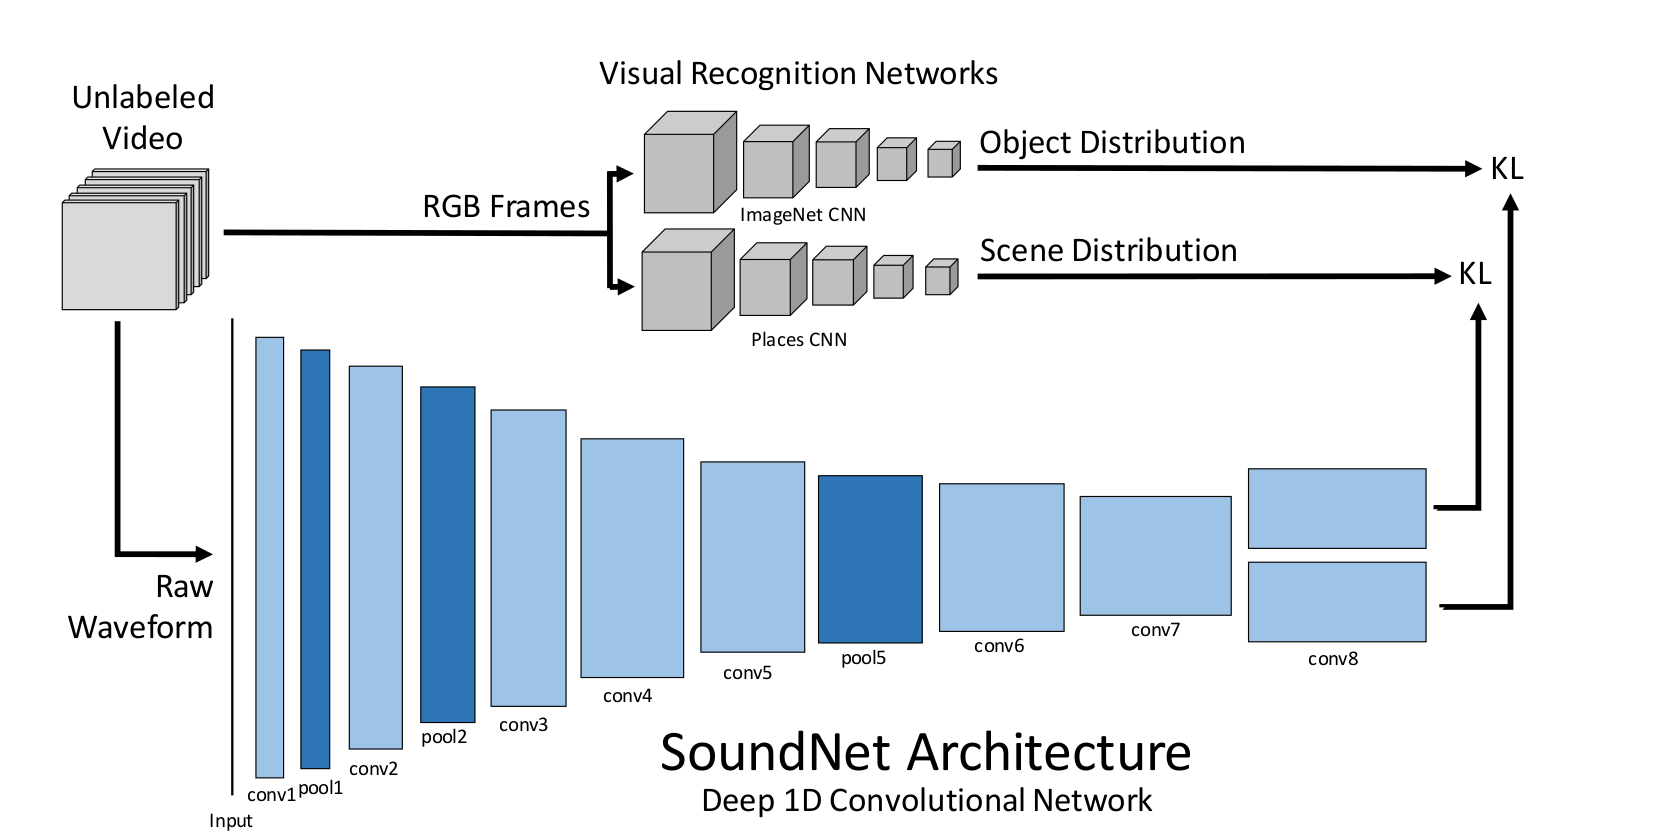
\includegraphics{../TP's/images/sound.jpeg}
\caption{sound.jpeg}
\end{figure}

    SoundNet is a deep convolutional network, layers are described as
follow:

\begin{enumerate}
\def\labelenumi{\arabic{enumi}.}
\item
  \texttt{Fully\ convolutional\ network:\ One\ dimensional\ convolutional\ layer\ +\ ReLU\ activation\ layer}\\
  \textbf{Why does it use convolutional layer into sound data?}

  Because they are translation invariant reducing the number of
  parameters and they allow stack layers, useful to detect higher-level
  concept.
\item
  \texttt{Pooling\ Layers}

  To down-sample variable length inputs.
\end{enumerate}

    \subsection{Math in training}\label{math-in-training}

Now it will be explained the maths behind this project. It is important
to emphasize that in training phase was used video, but the aim is to
recognize sounds. For this reason, in the compiled model videos are not
the input.

The problem has been modeled from a student-teacher perspective. In this
case, well-established networks for vision will teach the network for
sound to recognize scenes and objects.

The inputs in the model are \textbf{raw audio} \(x_i \in \mathcal{R}^D\)
and \textbf{video} \(y_i \in \mathcal{R}^{3xTxWxH}\) for each
\textbf{\(i\)} in \(1<i<N\), where \(W,H,T\) are width, height and
number of sampled frames in the video, respectively.

During learning the focus is get the probabilities \(g_k(y_i)\) from the
teacher vision network in order to train the student audio network
\(f_k(x_i)\), \textbf{\(k\)} enumerates the number of concepts
transfered from teacher to student.

In this way, they have defined a loss function,
\[L(g_k,f_k)=min_{\theta}\sum_{k=1}^K \sum_{i=1}^N D_{KL}(g_k(y_i)||f_k(x_i;\theta))\]
where \(D_{KL}(P||Q) = \sum_{j=1} P_j*log\frac{P_j}{Q_j}\) is the
Kullback--Leibler divergence.

That is a measure of how one probability distribution is different from
a second. The autors chose KL-divergence because is differentiable, then
it is possible optimize it using back-propagation and stochastic
gradient descent.

    \subsection{Key aspects of the learning
setting}\label{key-aspects-of-the-learning-setting}

\subsubsection{SOUND CLASSIFICATION}\label{sound-classification}

The authors use train SoundNet to classify visual categories but some
categories they wish to recognize may not appear in visual models. To
solve this problem they ignore the output of the network and use a
hidden representation as a strategy to attach semantic meaning to sound.
Using this internal representation they train a linear \textbf{SVM}
classifier considering a small number of labels about interest topics.

\begin{quote}
Another parameters from classifier. * Optimizer: Adam (learning rate of
0.001 and momentum term of 0.9). * Multi-class classification: one vs.
all. * Margin regularization: cross-validation. * Robustness: Standard
data augmentation.
\end{quote}

    \section{IMPLEMENTATION}\label{implementation}

\subsubsection{Code: model pre-trained}\label{code-model-pre-trained}

In this section will be explained the code and how it works.

The code given by the professor staff corresponds to
\href{https://github.com/brain-bzh/soundnet_keras}{SoundNet} built in
Keras with a pre-trained \textbf{8-layer model} originally obtained in
Torch 7.

\begin{quote}
Model parameters were obtained after 100.000 iterations (1 day GPU
processing) using 2M unlabeled videos and 140.000 videos to validation.
\end{quote}

\section{TODO}\label{todo}

Esquema

model trained with VGG16 (401 categories)

To start is necessary obtain a model with all parameters pre-trained
(weights, biases, etc.).

    \begin{Verbatim}[commandchars=\\\{\}]
{\color{incolor}In [{\color{incolor}1}]:} \PY{c+c1}{\PYZsh{} \PYZhy{}*\PYZhy{} coding: utf\PYZhy{}8 \PYZhy{}*\PYZhy{}}
        \PY{k+kn}{from} \PY{n+nn}{keras}\PY{n+nn}{.}\PY{n+nn}{layers} \PY{k}{import} \PY{n}{BatchNormalization}\PY{p}{,} \PY{n}{Activation}\PY{p}{,} \PY{n}{Conv1D}\PY{p}{,} \PY{n}{MaxPooling1D}\PY{p}{,} \PY{n}{ZeroPadding1D}\PY{p}{,} \PY{n}{InputLayer}
        \PY{k+kn}{from} \PY{n+nn}{keras}\PY{n+nn}{.}\PY{n+nn}{models} \PY{k}{import} \PY{n}{Sequential}
        \PY{k+kn}{import} \PY{n+nn}{numpy} \PY{k}{as} \PY{n+nn}{np}
        \PY{k+kn}{import} \PY{n+nn}{matplotlib}\PY{n+nn}{.}\PY{n+nn}{pyplot} \PY{k}{as} \PY{n+nn}{plt}
        \PY{k+kn}{import} \PY{n+nn}{librosa} \PY{c+c1}{\PYZsh{}audio library}
\end{Verbatim}


    \begin{Verbatim}[commandchars=\\\{\}]
Using TensorFlow backend.
/homes/d18arias/.local/lib/python3.6/site-packages/numba/errors.py:104: UserWarning: Insufficiently recent colorama version found. Numba requires colorama >= 0.3.9
  warnings.warn(msg)

    \end{Verbatim}

    \section{The configuration of the
layers}\label{the-configuration-of-the-layers}

With \texttt{build\_model} is built SoundNet according to the structure
defined by the authors. This model has as input the audio raw waveform
and two outputs: scenes and objects distribution.

    \begin{Verbatim}[commandchars=\\\{\}]
{\color{incolor}In [{\color{incolor}2}]:} \PY{k}{def} \PY{n+nf}{build\PYZus{}model}\PY{p}{(}\PY{p}{)}\PY{p}{:}
            \PY{l+s+sd}{\PYZdq{}\PYZdq{}\PYZdq{}}
        \PY{l+s+sd}{    Builds up the SoundNet model and loads the weights from a given model file (8\PYZhy{}layer model is stored at models/sound8.npy).}
        \PY{l+s+sd}{    :return: The model built according to architecture and weights pre\PYZhy{}stablished      }
        \PY{l+s+sd}{    \PYZdq{}\PYZdq{}\PYZdq{}}
            \PY{n}{model\PYZus{}weights} \PY{o}{=} \PY{n}{np}\PY{o}{.}\PY{n}{load}\PY{p}{(}\PY{l+s+s1}{\PYZsq{}}\PY{l+s+s1}{../soundnet\PYZus{}keras\PYZhy{}master/models/sound8.npy}\PY{l+s+s1}{\PYZsq{}}\PY{p}{,}\PY{n}{encoding} \PY{o}{=} \PY{l+s+s1}{\PYZsq{}}\PY{l+s+s1}{latin1}\PY{l+s+s1}{\PYZsq{}}\PY{p}{)}\PY{o}{.}\PY{n}{item}\PY{p}{(}\PY{p}{)}
            \PY{n}{model} \PY{o}{=} \PY{n}{Sequential}\PY{p}{(}\PY{p}{)}
            \PY{c+c1}{\PYZsh{}Input layer: audio raw waveform (1,length\PYZus{}audio,1)}
            \PY{n}{model}\PY{o}{.}\PY{n}{add}\PY{p}{(}\PY{n}{InputLayer}\PY{p}{(}\PY{n}{batch\PYZus{}input\PYZus{}shape}\PY{o}{=}\PY{p}{(}\PY{l+m+mi}{1}\PY{p}{,} \PY{k+kc}{None}\PY{p}{,} \PY{l+m+mi}{1}\PY{p}{)}\PY{p}{)}\PY{p}{)}
        
            \PY{n}{filter\PYZus{}parameters} \PY{o}{=} \PY{p}{[}\PY{p}{\PYZob{}}\PY{l+s+s1}{\PYZsq{}}\PY{l+s+s1}{name}\PY{l+s+s1}{\PYZsq{}}\PY{p}{:} \PY{l+s+s1}{\PYZsq{}}\PY{l+s+s1}{conv1}\PY{l+s+s1}{\PYZsq{}}\PY{p}{,} \PY{l+s+s1}{\PYZsq{}}\PY{l+s+s1}{num\PYZus{}filters}\PY{l+s+s1}{\PYZsq{}}\PY{p}{:} \PY{l+m+mi}{16}\PY{p}{,} \PY{l+s+s1}{\PYZsq{}}\PY{l+s+s1}{padding}\PY{l+s+s1}{\PYZsq{}}\PY{p}{:} \PY{l+m+mi}{32}\PY{p}{,}
                                  \PY{l+s+s1}{\PYZsq{}}\PY{l+s+s1}{kernel\PYZus{}size}\PY{l+s+s1}{\PYZsq{}}\PY{p}{:} \PY{l+m+mi}{64}\PY{p}{,} \PY{l+s+s1}{\PYZsq{}}\PY{l+s+s1}{conv\PYZus{}strides}\PY{l+s+s1}{\PYZsq{}}\PY{p}{:} \PY{l+m+mi}{2}\PY{p}{,}
                                  \PY{l+s+s1}{\PYZsq{}}\PY{l+s+s1}{pool\PYZus{}size}\PY{l+s+s1}{\PYZsq{}}\PY{p}{:} \PY{l+m+mi}{8}\PY{p}{,} \PY{l+s+s1}{\PYZsq{}}\PY{l+s+s1}{pool\PYZus{}strides}\PY{l+s+s1}{\PYZsq{}}\PY{p}{:} \PY{l+m+mi}{8}\PY{p}{\PYZcb{}}\PY{p}{,} \PY{c+c1}{\PYZsh{}pool1}
        
                                 \PY{p}{\PYZob{}}\PY{l+s+s1}{\PYZsq{}}\PY{l+s+s1}{name}\PY{l+s+s1}{\PYZsq{}}\PY{p}{:} \PY{l+s+s1}{\PYZsq{}}\PY{l+s+s1}{conv2}\PY{l+s+s1}{\PYZsq{}}\PY{p}{,} \PY{l+s+s1}{\PYZsq{}}\PY{l+s+s1}{num\PYZus{}filters}\PY{l+s+s1}{\PYZsq{}}\PY{p}{:} \PY{l+m+mi}{32}\PY{p}{,} \PY{l+s+s1}{\PYZsq{}}\PY{l+s+s1}{padding}\PY{l+s+s1}{\PYZsq{}}\PY{p}{:} \PY{l+m+mi}{16}\PY{p}{,}
                                  \PY{l+s+s1}{\PYZsq{}}\PY{l+s+s1}{kernel\PYZus{}size}\PY{l+s+s1}{\PYZsq{}}\PY{p}{:} \PY{l+m+mi}{32}\PY{p}{,} \PY{l+s+s1}{\PYZsq{}}\PY{l+s+s1}{conv\PYZus{}strides}\PY{l+s+s1}{\PYZsq{}}\PY{p}{:} \PY{l+m+mi}{2}\PY{p}{,}
                                  \PY{l+s+s1}{\PYZsq{}}\PY{l+s+s1}{pool\PYZus{}size}\PY{l+s+s1}{\PYZsq{}}\PY{p}{:} \PY{l+m+mi}{8}\PY{p}{,} \PY{l+s+s1}{\PYZsq{}}\PY{l+s+s1}{pool\PYZus{}strides}\PY{l+s+s1}{\PYZsq{}}\PY{p}{:} \PY{l+m+mi}{8}\PY{p}{\PYZcb{}}\PY{p}{,} \PY{c+c1}{\PYZsh{}pool2}
        
                                 \PY{p}{\PYZob{}}\PY{l+s+s1}{\PYZsq{}}\PY{l+s+s1}{name}\PY{l+s+s1}{\PYZsq{}}\PY{p}{:} \PY{l+s+s1}{\PYZsq{}}\PY{l+s+s1}{conv3}\PY{l+s+s1}{\PYZsq{}}\PY{p}{,} \PY{l+s+s1}{\PYZsq{}}\PY{l+s+s1}{num\PYZus{}filters}\PY{l+s+s1}{\PYZsq{}}\PY{p}{:} \PY{l+m+mi}{64}\PY{p}{,} \PY{l+s+s1}{\PYZsq{}}\PY{l+s+s1}{padding}\PY{l+s+s1}{\PYZsq{}}\PY{p}{:} \PY{l+m+mi}{8}\PY{p}{,}
                                  \PY{l+s+s1}{\PYZsq{}}\PY{l+s+s1}{kernel\PYZus{}size}\PY{l+s+s1}{\PYZsq{}}\PY{p}{:} \PY{l+m+mi}{16}\PY{p}{,} \PY{l+s+s1}{\PYZsq{}}\PY{l+s+s1}{conv\PYZus{}strides}\PY{l+s+s1}{\PYZsq{}}\PY{p}{:} \PY{l+m+mi}{2}\PY{p}{\PYZcb{}}\PY{p}{,}
        
                                 \PY{p}{\PYZob{}}\PY{l+s+s1}{\PYZsq{}}\PY{l+s+s1}{name}\PY{l+s+s1}{\PYZsq{}}\PY{p}{:} \PY{l+s+s1}{\PYZsq{}}\PY{l+s+s1}{conv4}\PY{l+s+s1}{\PYZsq{}}\PY{p}{,} \PY{l+s+s1}{\PYZsq{}}\PY{l+s+s1}{num\PYZus{}filters}\PY{l+s+s1}{\PYZsq{}}\PY{p}{:} \PY{l+m+mi}{128}\PY{p}{,} \PY{l+s+s1}{\PYZsq{}}\PY{l+s+s1}{padding}\PY{l+s+s1}{\PYZsq{}}\PY{p}{:} \PY{l+m+mi}{4}\PY{p}{,}
                                  \PY{l+s+s1}{\PYZsq{}}\PY{l+s+s1}{kernel\PYZus{}size}\PY{l+s+s1}{\PYZsq{}}\PY{p}{:} \PY{l+m+mi}{8}\PY{p}{,} \PY{l+s+s1}{\PYZsq{}}\PY{l+s+s1}{conv\PYZus{}strides}\PY{l+s+s1}{\PYZsq{}}\PY{p}{:} \PY{l+m+mi}{2}\PY{p}{\PYZcb{}}\PY{p}{,}
        
                                 \PY{p}{\PYZob{}}\PY{l+s+s1}{\PYZsq{}}\PY{l+s+s1}{name}\PY{l+s+s1}{\PYZsq{}}\PY{p}{:} \PY{l+s+s1}{\PYZsq{}}\PY{l+s+s1}{conv5}\PY{l+s+s1}{\PYZsq{}}\PY{p}{,} \PY{l+s+s1}{\PYZsq{}}\PY{l+s+s1}{num\PYZus{}filters}\PY{l+s+s1}{\PYZsq{}}\PY{p}{:} \PY{l+m+mi}{256}\PY{p}{,} \PY{l+s+s1}{\PYZsq{}}\PY{l+s+s1}{padding}\PY{l+s+s1}{\PYZsq{}}\PY{p}{:} \PY{l+m+mi}{2}\PY{p}{,}
                                  \PY{l+s+s1}{\PYZsq{}}\PY{l+s+s1}{kernel\PYZus{}size}\PY{l+s+s1}{\PYZsq{}}\PY{p}{:} \PY{l+m+mi}{4}\PY{p}{,} \PY{l+s+s1}{\PYZsq{}}\PY{l+s+s1}{conv\PYZus{}strides}\PY{l+s+s1}{\PYZsq{}}\PY{p}{:} \PY{l+m+mi}{2}\PY{p}{,}
                                  \PY{l+s+s1}{\PYZsq{}}\PY{l+s+s1}{pool\PYZus{}size}\PY{l+s+s1}{\PYZsq{}}\PY{p}{:} \PY{l+m+mi}{4}\PY{p}{,} \PY{l+s+s1}{\PYZsq{}}\PY{l+s+s1}{pool\PYZus{}strides}\PY{l+s+s1}{\PYZsq{}}\PY{p}{:} \PY{l+m+mi}{4}\PY{p}{\PYZcb{}}\PY{p}{,} \PY{c+c1}{\PYZsh{}pool5}
        
                                 \PY{p}{\PYZob{}}\PY{l+s+s1}{\PYZsq{}}\PY{l+s+s1}{name}\PY{l+s+s1}{\PYZsq{}}\PY{p}{:} \PY{l+s+s1}{\PYZsq{}}\PY{l+s+s1}{conv6}\PY{l+s+s1}{\PYZsq{}}\PY{p}{,} \PY{l+s+s1}{\PYZsq{}}\PY{l+s+s1}{num\PYZus{}filters}\PY{l+s+s1}{\PYZsq{}}\PY{p}{:} \PY{l+m+mi}{512}\PY{p}{,} \PY{l+s+s1}{\PYZsq{}}\PY{l+s+s1}{padding}\PY{l+s+s1}{\PYZsq{}}\PY{p}{:} \PY{l+m+mi}{2}\PY{p}{,}
                                  \PY{l+s+s1}{\PYZsq{}}\PY{l+s+s1}{kernel\PYZus{}size}\PY{l+s+s1}{\PYZsq{}}\PY{p}{:} \PY{l+m+mi}{4}\PY{p}{,} \PY{l+s+s1}{\PYZsq{}}\PY{l+s+s1}{conv\PYZus{}strides}\PY{l+s+s1}{\PYZsq{}}\PY{p}{:} \PY{l+m+mi}{2}\PY{p}{\PYZcb{}}\PY{p}{,}
        
                                 \PY{p}{\PYZob{}}\PY{l+s+s1}{\PYZsq{}}\PY{l+s+s1}{name}\PY{l+s+s1}{\PYZsq{}}\PY{p}{:} \PY{l+s+s1}{\PYZsq{}}\PY{l+s+s1}{conv7}\PY{l+s+s1}{\PYZsq{}}\PY{p}{,} \PY{l+s+s1}{\PYZsq{}}\PY{l+s+s1}{num\PYZus{}filters}\PY{l+s+s1}{\PYZsq{}}\PY{p}{:} \PY{l+m+mi}{1024}\PY{p}{,} \PY{l+s+s1}{\PYZsq{}}\PY{l+s+s1}{padding}\PY{l+s+s1}{\PYZsq{}}\PY{p}{:} \PY{l+m+mi}{2}\PY{p}{,}
                                  \PY{l+s+s1}{\PYZsq{}}\PY{l+s+s1}{kernel\PYZus{}size}\PY{l+s+s1}{\PYZsq{}}\PY{p}{:} \PY{l+m+mi}{4}\PY{p}{,} \PY{l+s+s1}{\PYZsq{}}\PY{l+s+s1}{conv\PYZus{}strides}\PY{l+s+s1}{\PYZsq{}}\PY{p}{:} \PY{l+m+mi}{2}\PY{p}{\PYZcb{}}\PY{p}{,}
        
                                 \PY{p}{\PYZob{}}\PY{l+s+s1}{\PYZsq{}}\PY{l+s+s1}{name}\PY{l+s+s1}{\PYZsq{}}\PY{p}{:} \PY{l+s+s1}{\PYZsq{}}\PY{l+s+s1}{conv8\PYZus{}2}\PY{l+s+s1}{\PYZsq{}}\PY{p}{,} \PY{l+s+s1}{\PYZsq{}}\PY{l+s+s1}{num\PYZus{}filters}\PY{l+s+s1}{\PYZsq{}}\PY{p}{:} \PY{l+m+mi}{401}\PY{p}{,} \PY{l+s+s1}{\PYZsq{}}\PY{l+s+s1}{padding}\PY{l+s+s1}{\PYZsq{}}\PY{p}{:} \PY{l+m+mi}{0}\PY{p}{,}
                                  \PY{l+s+s1}{\PYZsq{}}\PY{l+s+s1}{kernel\PYZus{}size}\PY{l+s+s1}{\PYZsq{}}\PY{p}{:} \PY{l+m+mi}{8}\PY{p}{,} \PY{l+s+s1}{\PYZsq{}}\PY{l+s+s1}{conv\PYZus{}strides}\PY{l+s+s1}{\PYZsq{}}\PY{p}{:} \PY{l+m+mi}{2}\PY{p}{\PYZcb{}}\PY{p}{,}\PY{c+c1}{\PYZsh{}output: VGG 401 classes}
                                 \PY{p}{]}
        
            \PY{k}{for} \PY{n}{x} \PY{o+ow}{in} \PY{n}{filter\PYZus{}parameters}\PY{p}{:}
                \PY{c+c1}{\PYZsh{}for each [zero\PYZus{}padding \PYZhy{} conv \PYZhy{} batchNormalization \PYZhy{} relu]}
                \PY{n}{model}\PY{o}{.}\PY{n}{add}\PY{p}{(}\PY{n}{ZeroPadding1D}\PY{p}{(}\PY{n}{padding}\PY{o}{=}\PY{n}{x}\PY{p}{[}\PY{l+s+s1}{\PYZsq{}}\PY{l+s+s1}{padding}\PY{l+s+s1}{\PYZsq{}}\PY{p}{]}\PY{p}{)}\PY{p}{)}
                \PY{n}{model}\PY{o}{.}\PY{n}{add}\PY{p}{(}\PY{n}{Conv1D}\PY{p}{(}\PY{n}{x}\PY{p}{[}\PY{l+s+s1}{\PYZsq{}}\PY{l+s+s1}{num\PYZus{}filters}\PY{l+s+s1}{\PYZsq{}}\PY{p}{]}\PY{p}{,}
                                 \PY{n}{kernel\PYZus{}size}\PY{o}{=}\PY{n}{x}\PY{p}{[}\PY{l+s+s1}{\PYZsq{}}\PY{l+s+s1}{kernel\PYZus{}size}\PY{l+s+s1}{\PYZsq{}}\PY{p}{]}\PY{p}{,}
                                 \PY{n}{strides}\PY{o}{=}\PY{n}{x}\PY{p}{[}\PY{l+s+s1}{\PYZsq{}}\PY{l+s+s1}{conv\PYZus{}strides}\PY{l+s+s1}{\PYZsq{}}\PY{p}{]}\PY{p}{,}
                                 \PY{n}{padding}\PY{o}{=}\PY{l+s+s1}{\PYZsq{}}\PY{l+s+s1}{valid}\PY{l+s+s1}{\PYZsq{}}\PY{p}{)}\PY{p}{)}
                \PY{n}{weights} \PY{o}{=} \PY{n}{model\PYZus{}weights}\PY{p}{[}\PY{n}{x}\PY{p}{[}\PY{l+s+s1}{\PYZsq{}}\PY{l+s+s1}{name}\PY{l+s+s1}{\PYZsq{}}\PY{p}{]}\PY{p}{]}\PY{p}{[}\PY{l+s+s1}{\PYZsq{}}\PY{l+s+s1}{weights}\PY{l+s+s1}{\PYZsq{}}\PY{p}{]}\PY{o}{.}\PY{n}{reshape}\PY{p}{(}\PY{n}{model}\PY{o}{.}\PY{n}{layers}\PY{p}{[}\PY{o}{\PYZhy{}}\PY{l+m+mi}{1}\PY{p}{]}\PY{o}{.}\PY{n}{get\PYZus{}weights}\PY{p}{(}\PY{p}{)}\PY{p}{[}\PY{l+m+mi}{0}\PY{p}{]}\PY{o}{.}\PY{n}{shape}\PY{p}{)}
                \PY{n}{biases} \PY{o}{=} \PY{n}{model\PYZus{}weights}\PY{p}{[}\PY{n}{x}\PY{p}{[}\PY{l+s+s1}{\PYZsq{}}\PY{l+s+s1}{name}\PY{l+s+s1}{\PYZsq{}}\PY{p}{]}\PY{p}{]}\PY{p}{[}\PY{l+s+s1}{\PYZsq{}}\PY{l+s+s1}{biases}\PY{l+s+s1}{\PYZsq{}}\PY{p}{]}
        
                \PY{n}{model}\PY{o}{.}\PY{n}{layers}\PY{p}{[}\PY{o}{\PYZhy{}}\PY{l+m+mi}{1}\PY{p}{]}\PY{o}{.}\PY{n}{set\PYZus{}weights}\PY{p}{(}\PY{p}{[}\PY{n}{weights}\PY{p}{,} \PY{n}{biases}\PY{p}{]}\PY{p}{)}  \PY{c+c1}{\PYZsh{}set weights in convolutional layer}
        
                \PY{k}{if} \PY{l+s+s1}{\PYZsq{}}\PY{l+s+s1}{conv8}\PY{l+s+s1}{\PYZsq{}} \PY{o+ow}{not} \PY{o+ow}{in} \PY{n}{x}\PY{p}{[}\PY{l+s+s1}{\PYZsq{}}\PY{l+s+s1}{name}\PY{l+s+s1}{\PYZsq{}}\PY{p}{]}\PY{p}{:}
                    \PY{n}{gamma} \PY{o}{=} \PY{n}{model\PYZus{}weights}\PY{p}{[}\PY{n}{x}\PY{p}{[}\PY{l+s+s1}{\PYZsq{}}\PY{l+s+s1}{name}\PY{l+s+s1}{\PYZsq{}}\PY{p}{]}\PY{p}{]}\PY{p}{[}\PY{l+s+s1}{\PYZsq{}}\PY{l+s+s1}{gamma}\PY{l+s+s1}{\PYZsq{}}\PY{p}{]}
                    \PY{n}{beta} \PY{o}{=} \PY{n}{model\PYZus{}weights}\PY{p}{[}\PY{n}{x}\PY{p}{[}\PY{l+s+s1}{\PYZsq{}}\PY{l+s+s1}{name}\PY{l+s+s1}{\PYZsq{}}\PY{p}{]}\PY{p}{]}\PY{p}{[}\PY{l+s+s1}{\PYZsq{}}\PY{l+s+s1}{beta}\PY{l+s+s1}{\PYZsq{}}\PY{p}{]}
                    \PY{n}{mean} \PY{o}{=} \PY{n}{model\PYZus{}weights}\PY{p}{[}\PY{n}{x}\PY{p}{[}\PY{l+s+s1}{\PYZsq{}}\PY{l+s+s1}{name}\PY{l+s+s1}{\PYZsq{}}\PY{p}{]}\PY{p}{]}\PY{p}{[}\PY{l+s+s1}{\PYZsq{}}\PY{l+s+s1}{mean}\PY{l+s+s1}{\PYZsq{}}\PY{p}{]}
                    \PY{n}{var} \PY{o}{=} \PY{n}{model\PYZus{}weights}\PY{p}{[}\PY{n}{x}\PY{p}{[}\PY{l+s+s1}{\PYZsq{}}\PY{l+s+s1}{name}\PY{l+s+s1}{\PYZsq{}}\PY{p}{]}\PY{p}{]}\PY{p}{[}\PY{l+s+s1}{\PYZsq{}}\PY{l+s+s1}{var}\PY{l+s+s1}{\PYZsq{}}\PY{p}{]}
        
                    
                    \PY{n}{model}\PY{o}{.}\PY{n}{add}\PY{p}{(}\PY{n}{BatchNormalization}\PY{p}{(}\PY{p}{)}\PY{p}{)}
                    \PY{n}{model}\PY{o}{.}\PY{n}{layers}\PY{p}{[}\PY{o}{\PYZhy{}}\PY{l+m+mi}{1}\PY{p}{]}\PY{o}{.}\PY{n}{set\PYZus{}weights}\PY{p}{(}\PY{p}{[}\PY{n}{gamma}\PY{p}{,} \PY{n}{beta}\PY{p}{,} \PY{n}{mean}\PY{p}{,} \PY{n}{var}\PY{p}{]}\PY{p}{)} \PY{c+c1}{\PYZsh{}set weights in batchNormalization}
                    \PY{n}{model}\PY{o}{.}\PY{n}{add}\PY{p}{(}\PY{n}{Activation}\PY{p}{(}\PY{l+s+s1}{\PYZsq{}}\PY{l+s+s1}{relu}\PY{l+s+s1}{\PYZsq{}}\PY{p}{)}\PY{p}{)}
                    
                \PY{k}{if} \PY{l+s+s1}{\PYZsq{}}\PY{l+s+s1}{pool\PYZus{}size}\PY{l+s+s1}{\PYZsq{}} \PY{o+ow}{in} \PY{n}{x}\PY{p}{:}
                    \PY{c+c1}{\PYZsh{}add 3 pooling layers}
                    \PY{n}{model}\PY{o}{.}\PY{n}{add}\PY{p}{(}\PY{n}{MaxPooling1D}\PY{p}{(}\PY{n}{pool\PYZus{}size}\PY{o}{=}\PY{n}{x}\PY{p}{[}\PY{l+s+s1}{\PYZsq{}}\PY{l+s+s1}{pool\PYZus{}size}\PY{l+s+s1}{\PYZsq{}}\PY{p}{]}\PY{p}{,}
                                           \PY{n}{strides}\PY{o}{=}\PY{n}{x}\PY{p}{[}\PY{l+s+s1}{\PYZsq{}}\PY{l+s+s1}{pool\PYZus{}strides}\PY{l+s+s1}{\PYZsq{}}\PY{p}{]}\PY{p}{,}
                                           \PY{n}{padding}\PY{o}{=}\PY{l+s+s1}{\PYZsq{}}\PY{l+s+s1}{valid}\PY{l+s+s1}{\PYZsq{}}\PY{p}{)}\PY{p}{)}
        
            \PY{k}{return} \PY{n}{model}
\end{Verbatim}


    \subsection{Audio preprocessing}\label{audio-preprocessing}

    \begin{Verbatim}[commandchars=\\\{\}]
{\color{incolor}In [{\color{incolor}3}]:} \PY{k}{def} \PY{n+nf}{preprocess}\PY{p}{(}\PY{n}{audio}\PY{p}{)}\PY{p}{:}
            \PY{n}{audio} \PY{o}{*}\PY{o}{=} \PY{l+m+mf}{256.0}  \PY{c+c1}{\PYZsh{} SoundNet requires an input range between \PYZhy{}256 and 256}
            \PY{c+c1}{\PYZsh{} reshaping the audio data, in this way it fits into the graph (batch\PYZus{}size, num\PYZus{}samples, num\PYZus{}filter\PYZus{}channels)}
            \PY{n}{audio} \PY{o}{=} \PY{n}{np}\PY{o}{.}\PY{n}{reshape}\PY{p}{(}\PY{n}{audio}\PY{p}{,} \PY{p}{(}\PY{l+m+mi}{1}\PY{p}{,} \PY{o}{\PYZhy{}}\PY{l+m+mi}{1}\PY{p}{,} \PY{l+m+mi}{1}\PY{p}{)}\PY{p}{)}
            \PY{k}{return} \PY{n}{audio}
        
        
        \PY{k}{def} \PY{n+nf}{load\PYZus{}audio}\PY{p}{(}\PY{n}{audio\PYZus{}file}\PY{p}{)}\PY{p}{:}
            \PY{n}{sample\PYZus{}rate} \PY{o}{=} \PY{l+m+mi}{22050}  \PY{c+c1}{\PYZsh{} SoundNet works on monophonic\PYZhy{}audio files with sample rate of 22050.}
            \PY{n}{audio}\PY{p}{,} \PY{n}{sr} \PY{o}{=} \PY{n}{librosa}\PY{o}{.}\PY{n}{load}\PY{p}{(}\PY{n}{audio\PYZus{}file}\PY{p}{,} \PY{n}{dtype}\PY{o}{=}\PY{l+s+s1}{\PYZsq{}}\PY{l+s+s1}{float32}\PY{l+s+s1}{\PYZsq{}}\PY{p}{,} \PY{n}{sr}\PY{o}{=}\PY{l+m+mi}{22050}\PY{p}{,} \PY{n}{mono}\PY{o}{=}\PY{k+kc}{True}\PY{p}{)} \PY{c+c1}{\PYZsh{}load audio}
            \PY{n}{audio} \PY{o}{=} \PY{n}{preprocess}\PY{p}{(}\PY{n}{audio}\PY{p}{)} \PY{c+c1}{\PYZsh{} pre\PYZhy{}process using SoundNet parameters}
            \PY{k}{return} \PY{n}{audio}
\end{Verbatim}


    \subsection{Construction of the model}\label{construction-of-the-model}

    \begin{Verbatim}[commandchars=\\\{\}]
{\color{incolor}In [{\color{incolor}4}]:} \PY{k+kn}{from} \PY{n+nn}{keras}\PY{n+nn}{.}\PY{n+nn}{utils} \PY{k}{import} \PY{n}{plot\PYZus{}model}
        
        \PY{c+c1}{\PYZsh{}Review of the model and architecture parameters}
        \PY{n}{model} \PY{o}{=} \PY{n}{build\PYZus{}model}\PY{p}{(}\PY{p}{)}
        \PY{n}{model}\PY{o}{.}\PY{n}{summary}\PY{p}{(}\PY{p}{)}
\end{Verbatim}


    \begin{Verbatim}[commandchars=\\\{\}]
\_\_\_\_\_\_\_\_\_\_\_\_\_\_\_\_\_\_\_\_\_\_\_\_\_\_\_\_\_\_\_\_\_\_\_\_\_\_\_\_\_\_\_\_\_\_\_\_\_\_\_\_\_\_\_\_\_\_\_\_\_\_\_\_\_
Layer (type)                 Output Shape              Param \#   
=================================================================
zero\_padding1d\_1 (ZeroPaddin (1, None, 1)              0         
\_\_\_\_\_\_\_\_\_\_\_\_\_\_\_\_\_\_\_\_\_\_\_\_\_\_\_\_\_\_\_\_\_\_\_\_\_\_\_\_\_\_\_\_\_\_\_\_\_\_\_\_\_\_\_\_\_\_\_\_\_\_\_\_\_
conv1d\_1 (Conv1D)            (1, None, 16)             1040      
\_\_\_\_\_\_\_\_\_\_\_\_\_\_\_\_\_\_\_\_\_\_\_\_\_\_\_\_\_\_\_\_\_\_\_\_\_\_\_\_\_\_\_\_\_\_\_\_\_\_\_\_\_\_\_\_\_\_\_\_\_\_\_\_\_
batch\_normalization\_1 (Batch (1, None, 16)             64        
\_\_\_\_\_\_\_\_\_\_\_\_\_\_\_\_\_\_\_\_\_\_\_\_\_\_\_\_\_\_\_\_\_\_\_\_\_\_\_\_\_\_\_\_\_\_\_\_\_\_\_\_\_\_\_\_\_\_\_\_\_\_\_\_\_
activation\_1 (Activation)    (1, None, 16)             0         
\_\_\_\_\_\_\_\_\_\_\_\_\_\_\_\_\_\_\_\_\_\_\_\_\_\_\_\_\_\_\_\_\_\_\_\_\_\_\_\_\_\_\_\_\_\_\_\_\_\_\_\_\_\_\_\_\_\_\_\_\_\_\_\_\_
max\_pooling1d\_1 (MaxPooling1 (1, None, 16)             0         
\_\_\_\_\_\_\_\_\_\_\_\_\_\_\_\_\_\_\_\_\_\_\_\_\_\_\_\_\_\_\_\_\_\_\_\_\_\_\_\_\_\_\_\_\_\_\_\_\_\_\_\_\_\_\_\_\_\_\_\_\_\_\_\_\_
zero\_padding1d\_2 (ZeroPaddin (1, None, 16)             0         
\_\_\_\_\_\_\_\_\_\_\_\_\_\_\_\_\_\_\_\_\_\_\_\_\_\_\_\_\_\_\_\_\_\_\_\_\_\_\_\_\_\_\_\_\_\_\_\_\_\_\_\_\_\_\_\_\_\_\_\_\_\_\_\_\_
conv1d\_2 (Conv1D)            (1, None, 32)             16416     
\_\_\_\_\_\_\_\_\_\_\_\_\_\_\_\_\_\_\_\_\_\_\_\_\_\_\_\_\_\_\_\_\_\_\_\_\_\_\_\_\_\_\_\_\_\_\_\_\_\_\_\_\_\_\_\_\_\_\_\_\_\_\_\_\_
batch\_normalization\_2 (Batch (1, None, 32)             128       
\_\_\_\_\_\_\_\_\_\_\_\_\_\_\_\_\_\_\_\_\_\_\_\_\_\_\_\_\_\_\_\_\_\_\_\_\_\_\_\_\_\_\_\_\_\_\_\_\_\_\_\_\_\_\_\_\_\_\_\_\_\_\_\_\_
activation\_2 (Activation)    (1, None, 32)             0         
\_\_\_\_\_\_\_\_\_\_\_\_\_\_\_\_\_\_\_\_\_\_\_\_\_\_\_\_\_\_\_\_\_\_\_\_\_\_\_\_\_\_\_\_\_\_\_\_\_\_\_\_\_\_\_\_\_\_\_\_\_\_\_\_\_
max\_pooling1d\_2 (MaxPooling1 (1, None, 32)             0         
\_\_\_\_\_\_\_\_\_\_\_\_\_\_\_\_\_\_\_\_\_\_\_\_\_\_\_\_\_\_\_\_\_\_\_\_\_\_\_\_\_\_\_\_\_\_\_\_\_\_\_\_\_\_\_\_\_\_\_\_\_\_\_\_\_
zero\_padding1d\_3 (ZeroPaddin (1, None, 32)             0         
\_\_\_\_\_\_\_\_\_\_\_\_\_\_\_\_\_\_\_\_\_\_\_\_\_\_\_\_\_\_\_\_\_\_\_\_\_\_\_\_\_\_\_\_\_\_\_\_\_\_\_\_\_\_\_\_\_\_\_\_\_\_\_\_\_
conv1d\_3 (Conv1D)            (1, None, 64)             32832     
\_\_\_\_\_\_\_\_\_\_\_\_\_\_\_\_\_\_\_\_\_\_\_\_\_\_\_\_\_\_\_\_\_\_\_\_\_\_\_\_\_\_\_\_\_\_\_\_\_\_\_\_\_\_\_\_\_\_\_\_\_\_\_\_\_
batch\_normalization\_3 (Batch (1, None, 64)             256       
\_\_\_\_\_\_\_\_\_\_\_\_\_\_\_\_\_\_\_\_\_\_\_\_\_\_\_\_\_\_\_\_\_\_\_\_\_\_\_\_\_\_\_\_\_\_\_\_\_\_\_\_\_\_\_\_\_\_\_\_\_\_\_\_\_
activation\_3 (Activation)    (1, None, 64)             0         
\_\_\_\_\_\_\_\_\_\_\_\_\_\_\_\_\_\_\_\_\_\_\_\_\_\_\_\_\_\_\_\_\_\_\_\_\_\_\_\_\_\_\_\_\_\_\_\_\_\_\_\_\_\_\_\_\_\_\_\_\_\_\_\_\_
zero\_padding1d\_4 (ZeroPaddin (1, None, 64)             0         
\_\_\_\_\_\_\_\_\_\_\_\_\_\_\_\_\_\_\_\_\_\_\_\_\_\_\_\_\_\_\_\_\_\_\_\_\_\_\_\_\_\_\_\_\_\_\_\_\_\_\_\_\_\_\_\_\_\_\_\_\_\_\_\_\_
conv1d\_4 (Conv1D)            (1, None, 128)            65664     
\_\_\_\_\_\_\_\_\_\_\_\_\_\_\_\_\_\_\_\_\_\_\_\_\_\_\_\_\_\_\_\_\_\_\_\_\_\_\_\_\_\_\_\_\_\_\_\_\_\_\_\_\_\_\_\_\_\_\_\_\_\_\_\_\_
batch\_normalization\_4 (Batch (1, None, 128)            512       
\_\_\_\_\_\_\_\_\_\_\_\_\_\_\_\_\_\_\_\_\_\_\_\_\_\_\_\_\_\_\_\_\_\_\_\_\_\_\_\_\_\_\_\_\_\_\_\_\_\_\_\_\_\_\_\_\_\_\_\_\_\_\_\_\_
activation\_4 (Activation)    (1, None, 128)            0         
\_\_\_\_\_\_\_\_\_\_\_\_\_\_\_\_\_\_\_\_\_\_\_\_\_\_\_\_\_\_\_\_\_\_\_\_\_\_\_\_\_\_\_\_\_\_\_\_\_\_\_\_\_\_\_\_\_\_\_\_\_\_\_\_\_
zero\_padding1d\_5 (ZeroPaddin (1, None, 128)            0         
\_\_\_\_\_\_\_\_\_\_\_\_\_\_\_\_\_\_\_\_\_\_\_\_\_\_\_\_\_\_\_\_\_\_\_\_\_\_\_\_\_\_\_\_\_\_\_\_\_\_\_\_\_\_\_\_\_\_\_\_\_\_\_\_\_
conv1d\_5 (Conv1D)            (1, None, 256)            131328    
\_\_\_\_\_\_\_\_\_\_\_\_\_\_\_\_\_\_\_\_\_\_\_\_\_\_\_\_\_\_\_\_\_\_\_\_\_\_\_\_\_\_\_\_\_\_\_\_\_\_\_\_\_\_\_\_\_\_\_\_\_\_\_\_\_
batch\_normalization\_5 (Batch (1, None, 256)            1024      
\_\_\_\_\_\_\_\_\_\_\_\_\_\_\_\_\_\_\_\_\_\_\_\_\_\_\_\_\_\_\_\_\_\_\_\_\_\_\_\_\_\_\_\_\_\_\_\_\_\_\_\_\_\_\_\_\_\_\_\_\_\_\_\_\_
activation\_5 (Activation)    (1, None, 256)            0         
\_\_\_\_\_\_\_\_\_\_\_\_\_\_\_\_\_\_\_\_\_\_\_\_\_\_\_\_\_\_\_\_\_\_\_\_\_\_\_\_\_\_\_\_\_\_\_\_\_\_\_\_\_\_\_\_\_\_\_\_\_\_\_\_\_
max\_pooling1d\_3 (MaxPooling1 (1, None, 256)            0         
\_\_\_\_\_\_\_\_\_\_\_\_\_\_\_\_\_\_\_\_\_\_\_\_\_\_\_\_\_\_\_\_\_\_\_\_\_\_\_\_\_\_\_\_\_\_\_\_\_\_\_\_\_\_\_\_\_\_\_\_\_\_\_\_\_
zero\_padding1d\_6 (ZeroPaddin (1, None, 256)            0         
\_\_\_\_\_\_\_\_\_\_\_\_\_\_\_\_\_\_\_\_\_\_\_\_\_\_\_\_\_\_\_\_\_\_\_\_\_\_\_\_\_\_\_\_\_\_\_\_\_\_\_\_\_\_\_\_\_\_\_\_\_\_\_\_\_
conv1d\_6 (Conv1D)            (1, None, 512)            524800    
\_\_\_\_\_\_\_\_\_\_\_\_\_\_\_\_\_\_\_\_\_\_\_\_\_\_\_\_\_\_\_\_\_\_\_\_\_\_\_\_\_\_\_\_\_\_\_\_\_\_\_\_\_\_\_\_\_\_\_\_\_\_\_\_\_
batch\_normalization\_6 (Batch (1, None, 512)            2048      
\_\_\_\_\_\_\_\_\_\_\_\_\_\_\_\_\_\_\_\_\_\_\_\_\_\_\_\_\_\_\_\_\_\_\_\_\_\_\_\_\_\_\_\_\_\_\_\_\_\_\_\_\_\_\_\_\_\_\_\_\_\_\_\_\_
activation\_6 (Activation)    (1, None, 512)            0         
\_\_\_\_\_\_\_\_\_\_\_\_\_\_\_\_\_\_\_\_\_\_\_\_\_\_\_\_\_\_\_\_\_\_\_\_\_\_\_\_\_\_\_\_\_\_\_\_\_\_\_\_\_\_\_\_\_\_\_\_\_\_\_\_\_
zero\_padding1d\_7 (ZeroPaddin (1, None, 512)            0         
\_\_\_\_\_\_\_\_\_\_\_\_\_\_\_\_\_\_\_\_\_\_\_\_\_\_\_\_\_\_\_\_\_\_\_\_\_\_\_\_\_\_\_\_\_\_\_\_\_\_\_\_\_\_\_\_\_\_\_\_\_\_\_\_\_
conv1d\_7 (Conv1D)            (1, None, 1024)           2098176   
\_\_\_\_\_\_\_\_\_\_\_\_\_\_\_\_\_\_\_\_\_\_\_\_\_\_\_\_\_\_\_\_\_\_\_\_\_\_\_\_\_\_\_\_\_\_\_\_\_\_\_\_\_\_\_\_\_\_\_\_\_\_\_\_\_
batch\_normalization\_7 (Batch (1, None, 1024)           4096      
\_\_\_\_\_\_\_\_\_\_\_\_\_\_\_\_\_\_\_\_\_\_\_\_\_\_\_\_\_\_\_\_\_\_\_\_\_\_\_\_\_\_\_\_\_\_\_\_\_\_\_\_\_\_\_\_\_\_\_\_\_\_\_\_\_
activation\_7 (Activation)    (1, None, 1024)           0         
\_\_\_\_\_\_\_\_\_\_\_\_\_\_\_\_\_\_\_\_\_\_\_\_\_\_\_\_\_\_\_\_\_\_\_\_\_\_\_\_\_\_\_\_\_\_\_\_\_\_\_\_\_\_\_\_\_\_\_\_\_\_\_\_\_
zero\_padding1d\_8 (ZeroPaddin (1, None, 1024)           0         
\_\_\_\_\_\_\_\_\_\_\_\_\_\_\_\_\_\_\_\_\_\_\_\_\_\_\_\_\_\_\_\_\_\_\_\_\_\_\_\_\_\_\_\_\_\_\_\_\_\_\_\_\_\_\_\_\_\_\_\_\_\_\_\_\_
conv1d\_8 (Conv1D)            (1, None, 401)            3285393   
=================================================================
Total params: 6,163,777
Trainable params: 6,159,713
Non-trainable params: 4,064
\_\_\_\_\_\_\_\_\_\_\_\_\_\_\_\_\_\_\_\_\_\_\_\_\_\_\_\_\_\_\_\_\_\_\_\_\_\_\_\_\_\_\_\_\_\_\_\_\_\_\_\_\_\_\_\_\_\_\_\_\_\_\_\_\_

    \end{Verbatim}

    \section{1. First experiments}\label{first-experiments}

At this moment, the SoundNet model is already built.

Next function is defined to obtain the output tags:

    \begin{Verbatim}[commandchars=\\\{\}]
{\color{incolor}In [{\color{incolor}5}]:} \PY{n}{f} \PY{o}{=} \PY{n+nb}{open}\PY{p}{(}\PY{l+s+s1}{\PYZsq{}}\PY{l+s+s1}{../soundnet\PYZus{}keras\PYZhy{}master/categories/categories\PYZus{}places2.txt}\PY{l+s+s1}{\PYZsq{}}\PY{p}{,} \PY{l+s+s1}{\PYZsq{}}\PY{l+s+s1}{r}\PY{l+s+s1}{\PYZsq{}}\PY{p}{)} 
        \PY{n}{categories} \PY{o}{=} \PY{n}{f}\PY{o}{.}\PY{n}{read}\PY{p}{(}\PY{p}{)}\PY{o}{.}\PY{n}{split}\PY{p}{(}\PY{l+s+s1}{\PYZsq{}}\PY{l+s+se}{\PYZbs{}n}\PY{l+s+s1}{\PYZsq{}}\PY{p}{)}
\end{Verbatim}


    \begin{Verbatim}[commandchars=\\\{\}]
{\color{incolor}In [{\color{incolor}6}]:} \PY{k}{def} \PY{n+nf}{predictions\PYZus{}to\PYZus{}scenes}\PY{p}{(}\PY{n}{prediction}\PY{p}{)}\PY{p}{:}
            \PY{n}{scenes} \PY{o}{=} \PY{p}{[}\PY{p}{]}
            \PY{k}{for} \PY{n}{p} \PY{o+ow}{in} \PY{n+nb}{range}\PY{p}{(}\PY{n}{prediction}\PY{o}{.}\PY{n}{shape}\PY{p}{[}\PY{l+m+mi}{1}\PY{p}{]}\PY{p}{)}\PY{p}{:}
                \PY{n}{scenes}\PY{o}{.}\PY{n}{append}\PY{p}{(}\PY{n}{categories}\PY{p}{[}\PY{n}{np}\PY{o}{.}\PY{n}{argmax}\PY{p}{(}\PY{n}{prediction}\PY{p}{[}\PY{l+m+mi}{0}\PY{p}{,} \PY{n}{p}\PY{p}{,} \PY{p}{:}\PY{p}{]}\PY{p}{)}\PY{p}{]}\PY{p}{)}
            \PY{k}{return} \PY{n}{scenes}
\end{Verbatim}


    \subsubsection{Input - Output SoundNet}\label{input---output-soundnet}

Which is the prediction?

    \begin{Verbatim}[commandchars=\\\{\}]
{\color{incolor}In [{\color{incolor}7}]:} \PY{c+c1}{\PYZsh{} let\PYZsq{}s load an audio file}
        \PY{n}{audiot}\PY{p}{,}\PY{n}{sr} \PY{o}{=} \PY{n}{librosa}\PY{o}{.}\PY{n}{load}\PY{p}{(}\PY{l+s+s1}{\PYZsq{}}\PY{l+s+s1}{../soundnet\PYZus{}keras\PYZhy{}master/railroad\PYZus{}audio.wav}\PY{l+s+s1}{\PYZsq{}}\PY{p}{,} 
                                 \PY{n}{dtype}\PY{o}{=}\PY{l+s+s1}{\PYZsq{}}\PY{l+s+s1}{float32}\PY{l+s+s1}{\PYZsq{}}\PY{p}{,} \PY{n}{sr}\PY{o}{=}\PY{l+m+mi}{22050}\PY{p}{,} \PY{n}{mono}\PY{o}{=}\PY{k+kc}{True}\PY{p}{)} \PY{c+c1}{\PYZsh{}load audio}
        
        \PY{c+c1}{\PYZsh{}library to listen sound}
        \PY{k+kn}{import} \PY{n+nn}{IPython}\PY{n+nn}{.}\PY{n+nn}{display} \PY{k}{as} \PY{n+nn}{ipd}
        \PY{n}{ipd}\PY{o}{.}\PY{n}{Audio}\PY{p}{(}\PY{n}{audiot}\PY{p}{,} \PY{n}{rate}\PY{o}{=}\PY{n}{sr}\PY{p}{)} \PY{c+c1}{\PYZsh{} load }
        
        \PY{c+c1}{\PYZsh{}sound like a railroad or not?}
\end{Verbatim}


\begin{Verbatim}[commandchars=\\\{\}]
{\color{outcolor}Out[{\color{outcolor}7}]:} <IPython.lib.display.Audio object>
\end{Verbatim}
            
    \begin{Verbatim}[commandchars=\\\{\}]
{\color{incolor}In [{\color{incolor}8}]:} \PY{c+c1}{\PYZsh{} Function to built the model and predict scenes related with a given audio }
        \PY{k}{def} \PY{n+nf}{predict\PYZus{}scene\PYZus{}from\PYZus{}audio\PYZus{}file}\PY{p}{(}\PY{n}{audio\PYZus{}file}\PY{p}{)}\PY{p}{:}
            \PY{n}{model} \PY{o}{=} \PY{n}{build\PYZus{}model}\PY{p}{(}\PY{p}{)}
            \PY{n}{audio} \PY{o}{=} \PY{n}{load\PYZus{}audio}\PY{p}{(}\PY{n}{audio\PYZus{}file}\PY{p}{)}
            \PY{k}{return} \PY{n}{model}\PY{o}{.}\PY{n}{predict}\PY{p}{(}\PY{n}{audio}\PY{p}{)}
        
        \PY{c+c1}{\PYZsh{} Use previous function to predict and show scenes in the audio}
        \PY{n}{prediction} \PY{o}{=} \PY{n}{predict\PYZus{}scene\PYZus{}from\PYZus{}audio\PYZus{}file}\PY{p}{(}\PY{l+s+s1}{\PYZsq{}}\PY{l+s+s1}{../soundnet\PYZus{}keras\PYZhy{}master/railroad\PYZus{}audio.wav}\PY{l+s+s1}{\PYZsq{}}\PY{p}{)}
        \PY{n+nb}{print}\PY{p}{(}\PY{l+s+s2}{\PYZdq{}}\PY{l+s+s2}{output model shape}\PY{l+s+s2}{\PYZdq{}}\PY{p}{,} \PY{n}{prediction}\PY{o}{.}\PY{n}{shape}\PY{p}{)}
\end{Verbatim}


    \begin{Verbatim}[commandchars=\\\{\}]
output model shape (1, 4, 401)

    \end{Verbatim}

    \subsubsection{We can see the different ways in which the classes were
activated, in a more detailed
manner:}\label{we-can-see-the-different-ways-in-which-the-classes-were-activated-in-a-more-detailed-manner}

    \begin{Verbatim}[commandchars=\\\{\}]
{\color{incolor}In [{\color{incolor}9}]:} \PY{k}{def} \PY{n+nf}{findMax}\PY{p}{(}\PY{n}{vector}\PY{p}{)}\PY{p}{:} \PY{c+c1}{\PYZsh{}find 3 classes max}
            \PY{n}{maximus} \PY{o}{=} \PY{p}{[}\PY{p}{]}
            \PY{k}{for} \PY{n}{i} \PY{o+ow}{in} \PY{n+nb}{range}\PY{p}{(}\PY{l+m+mi}{3}\PY{p}{)}\PY{p}{:}
                \PY{n}{index} \PY{o}{=} \PY{n}{np}\PY{o}{.}\PY{n}{argmax}\PY{p}{(}\PY{n}{vector}\PY{p}{)}
                \PY{n}{f} \PY{o}{=} \PY{p}{[}\PY{n}{index}\PY{p}{,} \PY{n+nb}{max}\PY{p}{(}\PY{n}{vector}\PY{p}{)}\PY{p}{]}
                \PY{n}{vector}\PY{p}{[}\PY{n}{index}\PY{p}{]} \PY{o}{=} \PY{l+m+mi}{0} 
                \PY{n}{maximus}\PY{o}{.}\PY{n}{append}\PY{p}{(}\PY{n}{f}\PY{p}{)}
            \PY{k}{return} \PY{n}{maximus}   
\end{Verbatim}


    \begin{Verbatim}[commandchars=\\\{\}]
{\color{incolor}In [{\color{incolor}10}]:} \PY{k}{def} \PY{n+nf}{putText}\PY{p}{(}\PY{n}{datos}\PY{p}{,}\PY{n}{x}\PY{p}{)}\PY{p}{:}
             \PY{n}{f} \PY{o}{=} \PY{n}{findMax}\PY{p}{(}\PY{n}{datos}\PY{p}{)}
             \PY{n}{text} \PY{o}{=} \PY{l+s+s2}{\PYZdq{}}\PY{l+s+s2}{Prediction }\PY{l+s+s2}{\PYZdq{}} \PY{o}{+} \PY{n+nb}{str}\PY{p}{(}\PY{n}{x}\PY{p}{)} \PY{o}{+} \PY{l+s+s2}{\PYZdq{}}\PY{l+s+s2}{: }\PY{l+s+s2}{\PYZdq{}}
             \PY{k}{for} \PY{n}{i} \PY{o+ow}{in} \PY{n}{f}\PY{p}{:}
                 \PY{n}{text} \PY{o}{=} \PY{n}{text} \PY{o}{+}\PY{l+s+s2}{\PYZdq{}}\PY{l+s+s2}{ \PYZhy{} }\PY{l+s+s2}{\PYZdq{}}\PY{o}{+} \PY{n}{categories}\PY{p}{[}\PY{n}{i}\PY{p}{[}\PY{l+m+mi}{0}\PY{p}{]}\PY{p}{]}
             \PY{n+nb}{print}\PY{p}{(}\PY{n}{text}\PY{p}{)}
\end{Verbatim}


    \begin{Verbatim}[commandchars=\\\{\}]
{\color{incolor}In [{\color{incolor}11}]:}  \PY{k}{def} \PY{n+nf}{plot\PYZus{}scenes}\PY{p}{(}\PY{n}{pred}\PY{p}{,}\PY{n}{title}\PY{p}{)}\PY{p}{:}
             \PY{n}{plt}\PY{o}{.}\PY{n}{figure}\PY{p}{(}\PY{n}{figsize}\PY{o}{=}\PY{p}{(}\PY{l+m+mi}{16}\PY{p}{,}\PY{l+m+mi}{8}\PY{p}{)}\PY{p}{)}
             \PY{k}{for} \PY{n}{i} \PY{o+ow}{in} \PY{n+nb}{range}\PY{p}{(}\PY{n}{pred}\PY{o}{.}\PY{n}{shape}\PY{p}{[}\PY{l+m+mi}{1}\PY{p}{]}\PY{p}{)}\PY{p}{:}\PY{c+c1}{\PYZsh{} number of prediction vectors}
                 \PY{n}{datos} \PY{o}{=} \PY{p}{(}\PY{n}{pred}\PY{p}{[}\PY{l+m+mi}{0}\PY{p}{,}\PY{n}{i}\PY{p}{,}\PY{p}{:}\PY{p}{]} \PY{o}{\PYZgt{}} \PY{l+m+mi}{0}\PY{p}{)}\PY{o}{*} \PY{n}{pred}\PY{p}{[}\PY{l+m+mi}{0}\PY{p}{,}\PY{n}{i}\PY{p}{,}\PY{p}{:}\PY{p}{]} \PY{c+c1}{\PYZsh{}find classes }
                 \PY{n}{label}\PY{o}{=}\PY{l+s+s1}{\PYZsq{}}\PY{l+s+s1}{Window no: }\PY{l+s+s1}{\PYZsq{}}\PY{o}{+} \PY{n+nb}{str}\PY{p}{(}\PY{n}{i}\PY{p}{)}
                 \PY{n}{plt}\PY{o}{.}\PY{n}{bar}\PY{p}{(}\PY{n}{np}\PY{o}{.}\PY{n}{arange}\PY{p}{(}\PY{l+m+mi}{0}\PY{p}{,}\PY{n}{pred}\PY{o}{.}\PY{n}{shape}\PY{p}{[}\PY{l+m+mi}{2}\PY{p}{]}\PY{p}{)}\PY{p}{,}\PY{n}{datos}\PY{p}{,}\PY{n}{label} \PY{o}{=} \PY{n}{label}\PY{p}{)} \PY{c+c1}{\PYZsh{} it draws the histogram for each window}
                 \PY{n}{m} \PY{o}{=} \PY{n}{np}\PY{o}{.}\PY{n}{argmax}\PY{p}{(}\PY{n}{datos}\PY{p}{)}
                 \PY{n}{plt}\PY{o}{.}\PY{n}{text}\PY{p}{(}\PY{n}{m}\PY{p}{,}\PY{n+nb}{max}\PY{p}{(}\PY{n}{datos}\PY{p}{)}\PY{o}{\PYZhy{}}\PY{p}{(}\PY{l+m+mf}{0.01}\PY{p}{)}\PY{p}{,}\PY{l+s+s1}{\PYZsq{}}\PY{l+s+s1}{Scene out: }\PY{l+s+s1}{\PYZsq{}}\PY{o}{+} \PY{n+nb}{str}\PY{p}{(}\PY{n}{i}\PY{p}{)} \PY{o}{+}\PY{n}{categories}\PY{p}{[}\PY{n}{m}\PY{p}{]}\PY{p}{)}   
                 \PY{n}{putText}\PY{p}{(}\PY{n}{datos}\PY{p}{,}\PY{n}{i}\PY{p}{)}
         
             \PY{n}{plt}\PY{o}{.}\PY{n}{legend}\PY{p}{(}\PY{p}{)}   
             \PY{n}{plt}\PY{o}{.}\PY{n}{title}\PY{p}{(}\PY{n}{title}\PY{p}{)}
             \PY{n}{plt}\PY{o}{.}\PY{n}{xlabel}\PY{p}{(}\PY{l+s+s1}{\PYZsq{}}\PY{l+s+s1}{Scenes}\PY{l+s+s1}{\PYZsq{}}\PY{p}{)}
\end{Verbatim}


    \begin{Verbatim}[commandchars=\\\{\}]
{\color{incolor}In [{\color{incolor}12}]:} \PY{c+c1}{\PYZsh{} Use previous function to show histogram in this first audio}
         \PY{n}{plot\PYZus{}scenes}\PY{p}{(}\PY{n}{prediction}\PY{p}{,}\PY{l+s+s1}{\PYZsq{}}\PY{l+s+s1}{Output railroad}\PY{l+s+s1}{\PYZsq{}}\PY{p}{)}
\end{Verbatim}


    \begin{Verbatim}[commandchars=\\\{\}]
Prediction 0:  - /r/railroad\_track - /t/train\_station/platform - /t/train\_railway
Prediction 1:  - /r/railroad\_track - /t/train\_station/platform - /t/train\_railway
Prediction 2:  - /r/railroad\_track - /t/train\_station/platform - /t/train\_railway
Prediction 3:  - /t/train\_station/platform - /r/railroad\_track - /t/train\_railway

    \end{Verbatim}

    \begin{center}
    \adjustimage{max size={0.9\linewidth}{0.9\paperheight}}{output_26_1.png}
    \end{center}
    { \hspace*{\fill} \\}
    
    \subsubsection{Experiment with another audio: school
yard}\label{experiment-with-another-audio-school-yard}

    \begin{Verbatim}[commandchars=\\\{\}]
{\color{incolor}In [{\color{incolor}13}]:} \PY{c+c1}{\PYZsh{} Repeat the process to obtain a new prediction}
         \PY{n}{prediction2} \PY{o}{=} \PY{n}{predict\PYZus{}scene\PYZus{}from\PYZus{}audio\PYZus{}file}\PY{p}{(}\PY{l+s+s1}{\PYZsq{}}\PY{l+s+s1}{../soundnet\PYZus{}keras\PYZhy{}master/school.wav}\PY{l+s+s1}{\PYZsq{}}\PY{p}{)}
         \PY{n+nb}{print}\PY{p}{(}\PY{l+s+s2}{\PYZdq{}}\PY{l+s+s2}{output model shape}\PY{l+s+s2}{\PYZdq{}}\PY{p}{,} \PY{n}{prediction2}\PY{o}{.}\PY{n}{shape}\PY{p}{)} \PY{c+c1}{\PYZsh{}output model }
\end{Verbatim}


    \begin{Verbatim}[commandchars=\\\{\}]
output model shape (1, 2, 401)

    \end{Verbatim}

    \begin{Verbatim}[commandchars=\\\{\}]
{\color{incolor}In [{\color{incolor}14}]:} \PY{n}{plot\PYZus{}scenes}\PY{p}{(}\PY{n}{prediction2}\PY{p}{,}\PY{l+s+s1}{\PYZsq{}}\PY{l+s+s1}{Output school yard}\PY{l+s+s1}{\PYZsq{}}\PY{p}{)}
\end{Verbatim}


    \begin{Verbatim}[commandchars=\\\{\}]
Prediction 0:  - /p/playground - /s/soccer\_field - /a/amusement\_park
Prediction 1:  - /p/playground - /s/soccer\_field - /b/baseball\_field

    \end{Verbatim}

    \begin{center}
    \adjustimage{max size={0.9\linewidth}{0.9\paperheight}}{output_29_1.png}
    \end{center}
    { \hspace*{\fill} \\}
    
    \begin{quote}
\section{Size minimum}\label{size-minimum}

The number of prediction vectors (output-size) depends on the size of
the input. It means input must have a minimum size to allow the model
predict some output. In the next lines, we try to find this frontier.
\end{quote}

    \begin{Verbatim}[commandchars=\\\{\}]
{\color{incolor}In [{\color{incolor}15}]:} \PY{c+c1}{\PYZsh{} Use previous function to predict and show scenes in the audio}
         \PY{n}{prediction} \PY{o}{=} \PY{n}{predict\PYZus{}scene\PYZus{}from\PYZus{}audio\PYZus{}file}\PY{p}{(}\PY{l+s+s1}{\PYZsq{}}\PY{l+s+s1}{../soundnet\PYZus{}keras\PYZhy{}master/railroad\PYZus{}audio.wav}\PY{l+s+s1}{\PYZsq{}}\PY{p}{)}
         \PY{n+nb}{print}\PY{p}{(}\PY{l+s+s2}{\PYZdq{}}\PY{l+s+s2}{output model shape}\PY{l+s+s2}{\PYZdq{}}\PY{p}{,} \PY{n}{prediction}\PY{o}{.}\PY{n}{shape}\PY{p}{)}
\end{Verbatim}


    \begin{Verbatim}[commandchars=\\\{\}]
output model shape (1, 4, 401)

    \end{Verbatim}

    \section{ESC -50 Dataset}\label{esc--50-dataset}

    The dataset ESC-50 is a collection of 2000 short (5 seconds) recordings
of environmental sounds from equally balanced 50 categories selected
from 5 major groups (animals, natural soundscapes, human non-speech
sounds, interior/domestic sounds, and exterior/urban noises).

In order to evaluate the model behavior we use the dataset ESC-10. It is
a subset of ESC-50 which consists of 10 classes (dog bark, rain, sea
waves, baby cry, clock tic, person sneeze, helicopter, chainsaw,
rooster, and fire cracking).

    \begin{Verbatim}[commandchars=\\\{\}]
{\color{incolor}In [{\color{incolor}16}]:} \PY{k+kn}{import} \PY{n+nn}{pandas} \PY{k}{as} \PY{n+nn}{pd}
         \PY{n}{test} \PY{o}{=} \PY{n}{pd}\PY{o}{.}\PY{n}{read\PYZus{}csv}\PY{p}{(}\PY{l+s+s1}{\PYZsq{}}\PY{l+s+s1}{../ESC\PYZhy{}50\PYZhy{}master/meta/esc50.csv}\PY{l+s+s1}{\PYZsq{}}\PY{p}{,}\PY{n}{sep}\PY{o}{=}\PY{l+s+s1}{\PYZsq{}}\PY{l+s+s1}{,}\PY{l+s+s1}{\PYZsq{}}\PY{p}{)}
         \PY{n}{test}\PY{o}{.}\PY{n}{head}\PY{p}{(}\PY{p}{)}
\end{Verbatim}


\begin{Verbatim}[commandchars=\\\{\}]
{\color{outcolor}Out[{\color{outcolor}16}]:}             filename  fold  target        category  esc10  src\_file take
         0   1-100032-A-0.wav     1       0             dog   True    100032    A
         1  1-100038-A-14.wav     1      14  chirping\_birds  False    100038    A
         2  1-100210-A-36.wav     1      36  vacuum\_cleaner  False    100210    A
         3  1-100210-B-36.wav     1      36  vacuum\_cleaner  False    100210    B
         4  1-101296-A-19.wav     1      19    thunderstorm  False    101296    A
\end{Verbatim}
            
    \begin{Verbatim}[commandchars=\\\{\}]
{\color{incolor}In [{\color{incolor}17}]:} \PY{c+c1}{\PYZsh{}only 10 classes}
         \PY{n}{esc10} \PY{o}{=} \PY{n}{test}\PY{p}{[} \PY{n}{test}\PY{p}{[}\PY{l+s+s1}{\PYZsq{}}\PY{l+s+s1}{esc10}\PY{l+s+s1}{\PYZsq{}}\PY{p}{]} \PY{o}{==} \PY{k+kc}{True}\PY{p}{]}
         \PY{n+nb}{print}\PY{p}{(}\PY{n}{esc10}\PY{p}{[}\PY{p}{:}\PY{l+m+mi}{5}\PY{p}{]}\PY{p}{)} \PY{c+c1}{\PYZsh{}first 5 elements}
\end{Verbatim}


    \begin{Verbatim}[commandchars=\\\{\}]
             filename  fold  target        category  esc10  src\_file take
0    1-100032-A-0.wav     1       0             dog   True    100032    A
14   1-110389-A-0.wav     1       0             dog   True    110389    A
24  1-116765-A-41.wav     1      41        chainsaw   True    116765    A
54   1-17150-A-12.wav     1      12  crackling\_fire   True     17150    A
55  1-172649-A-40.wav     1      40      helicopter   True    172649    A

    \end{Verbatim}

    \begin{Verbatim}[commandchars=\\\{\}]
{\color{incolor}In [{\color{incolor}18}]:} \PY{n}{data} \PY{o}{=} \PY{p}{[}\PY{p}{]} \PY{c+c1}{\PYZsh{}load the audiofiles}
         \PY{n}{list\PYZus{}target} \PY{o}{=} \PY{n}{esc10}\PY{p}{[}\PY{l+s+s1}{\PYZsq{}}\PY{l+s+s1}{target}\PY{l+s+s1}{\PYZsq{}}\PY{p}{]}
         \PY{n}{list\PYZus{}category} \PY{o}{=} \PY{n}{esc10}\PY{p}{[}\PY{l+s+s1}{\PYZsq{}}\PY{l+s+s1}{category}\PY{l+s+s1}{\PYZsq{}}\PY{p}{]}
         
         \PY{k}{for} \PY{n}{file\PYZus{}name} \PY{o+ow}{in} \PY{n+nb}{list}\PY{p}{(}\PY{n}{esc10}\PY{p}{[}\PY{l+s+s1}{\PYZsq{}}\PY{l+s+s1}{filename}\PY{l+s+s1}{\PYZsq{}}\PY{p}{]}\PY{p}{)}\PY{p}{:}
             \PY{n}{audio} \PY{o}{=} \PY{n}{load\PYZus{}audio}\PY{p}{(}\PY{l+s+s1}{\PYZsq{}}\PY{l+s+s1}{../ESC\PYZhy{}50\PYZhy{}master/audio/}\PY{l+s+s1}{\PYZsq{}}\PY{o}{+}\PY{n}{file\PYZus{}name}\PY{p}{)}
             \PY{n}{data}\PY{o}{.}\PY{n}{append}\PY{p}{(}\PY{n}{audio}\PY{p}{)}
          
\end{Verbatim}


    \begin{Verbatim}[commandchars=\\\{\}]
{\color{incolor}In [{\color{incolor}19}]:} \PY{n+nb}{print}\PY{p}{(}\PY{n+nb}{len}\PY{p}{(}\PY{n}{data}\PY{p}{)}\PY{p}{,}\PY{n+nb}{len}\PY{p}{(}\PY{n}{list\PYZus{}target}\PY{p}{)}\PY{p}{,}\PY{n+nb}{len}\PY{p}{(}\PY{n}{list\PYZus{}category}\PY{p}{)}\PY{p}{)} \PY{c+c1}{\PYZsh{}load correctly}
         \PY{n+nb}{print}\PY{p}{(}\PY{n}{list\PYZus{}target}\PY{p}{[}\PY{l+m+mi}{0}\PY{p}{]}\PY{p}{,}\PY{n}{list\PYZus{}category}\PY{p}{[}\PY{l+m+mi}{0}\PY{p}{]}\PY{p}{)} \PY{c+c1}{\PYZsh{}load correctly}
\end{Verbatim}


    \begin{Verbatim}[commandchars=\\\{\}]
400 400 400
0 dog

    \end{Verbatim}

    \subsubsection{Test with Esc10}\label{test-with-esc10}

    \begin{Verbatim}[commandchars=\\\{\}]
{\color{incolor}In [{\color{incolor}20}]:} \PY{n}{datos} \PY{o}{=} \PY{n}{np}\PY{o}{.}\PY{n}{asarray}\PY{p}{(}\PY{p}{[}\PY{n}{data}\PY{p}{[}\PY{l+m+mi}{155}\PY{p}{]}\PY{p}{]}\PY{p}{)}\PY{o}{.}\PY{n}{reshape}\PY{p}{(}\PY{l+m+mi}{1}\PY{p}{,}\PY{o}{\PYZhy{}}\PY{l+m+mi}{1}\PY{p}{,}\PY{l+m+mi}{1}\PY{p}{)} \PY{c+c1}{\PYZsh{} failure due to the size}
         \PY{n+nb}{print}\PY{p}{(}\PY{n}{datos}\PY{o}{.}\PY{n}{shape}\PY{p}{)}
\end{Verbatim}


    \begin{Verbatim}[commandchars=\\\{\}]
(1, 110250, 1)

    \end{Verbatim}

    \begin{quote}
\textbf{Compilation error}: the audio has a duration of 5s (110250
samples / 22050 samples per second). The model does not have the minimum
number of required samples and is reflected in the Keras kernel. It
turns off because of this error.
\end{quote}

    \begin{Verbatim}[commandchars=\\\{\}]
{\color{incolor}In [{\color{incolor}21}]:} \PY{c+c1}{\PYZsh{}p = model.predict(datos) \PYZsh{}\PYZhy{}\PYZhy{}\PYZhy{}\PYZhy{}\PYZhy{}\PYZhy{}\PYZhy{}\PYZhy{}\PYZhy{}\PYZhy{}\PYZhy{} error (last layer \PYZhy{} output)}
         \PY{c+c1}{\PYZsh{}print(p.shape)           \PYZsh{}\PYZhy{}\PYZhy{}\PYZhy{}\PYZhy{}\PYZhy{}\PYZhy{}\PYZhy{}\PYZhy{}\PYZhy{}\PYZhy{}\PYZhy{} error}
\end{Verbatim}


    A new raw audio with three(3) times concatenate single audio is enough
in terms of samples for the model.

    \begin{Verbatim}[commandchars=\\\{\}]
{\color{incolor}In [{\color{incolor}22}]:} \PY{c+c1}{\PYZsh{}For this test we use \PYZdq{}audio 1\PYZhy{}172649\PYZhy{}b\PYZhy{}40 helicopter\PYZdq{} audio number 5 in datos}
         \PY{n}{datos} \PY{o}{=} \PY{n}{np}\PY{o}{.}\PY{n}{asarray}\PY{p}{(}\PY{p}{[}\PY{n}{data}\PY{p}{[}\PY{l+m+mi}{5}\PY{p}{]}\PY{p}{,}\PY{n}{data}\PY{p}{[}\PY{l+m+mi}{5}\PY{p}{]}\PY{p}{,}\PY{n}{data}\PY{p}{[}\PY{l+m+mi}{5}\PY{p}{]}\PY{p}{]}\PY{p}{)}\PY{o}{.}\PY{n}{reshape}\PY{p}{(}\PY{l+m+mi}{1}\PY{p}{,}\PY{o}{\PYZhy{}}\PY{l+m+mi}{1}\PY{p}{,}\PY{l+m+mi}{1}\PY{p}{)}
         \PY{n+nb}{print}\PY{p}{(}\PY{l+s+s2}{\PYZdq{}}\PY{l+s+s2}{input shape}\PY{l+s+s2}{\PYZdq{}}\PY{p}{,} \PY{n}{datos}\PY{o}{.}\PY{n}{shape}\PY{p}{)}
\end{Verbatim}


    \begin{Verbatim}[commandchars=\\\{\}]
input shape (1, 330750, 1)

    \end{Verbatim}

    \begin{Verbatim}[commandchars=\\\{\}]
{\color{incolor}In [{\color{incolor}23}]:} \PY{n}{p} \PY{o}{=} \PY{n}{model}\PY{o}{.}\PY{n}{predict}\PY{p}{(}\PY{n}{datos}\PY{p}{)} \PY{c+c1}{\PYZsh{}\PYZhy{} \PYZgt{} Three times data: enough samples for the model}
         \PY{n+nb}{print}\PY{p}{(}\PY{l+s+s2}{\PYZdq{}}\PY{l+s+s2}{output shape}\PY{l+s+s2}{\PYZdq{}}\PY{p}{,}\PY{n}{p}\PY{o}{.}\PY{n}{shape}\PY{p}{)}
         \PY{n}{plot\PYZus{}scenes}\PY{p}{(}\PY{n}{p}\PY{p}{,}\PY{l+s+s1}{\PYZsq{}}\PY{l+s+s1}{output esc10\PYZhy{}helicopter}\PY{l+s+s1}{\PYZsq{}}\PY{p}{)}
\end{Verbatim}


    \begin{Verbatim}[commandchars=\\\{\}]
output shape (1, 2, 401)
Prediction 0:  - /p/parking\_lot - /r/runway - /r/raceway
Prediction 1:  - /r/runway - /p/parking\_lot - /r/raceway

    \end{Verbatim}

    \begin{center}
    \adjustimage{max size={0.9\linewidth}{0.9\paperheight}}{output_44_1.png}
    \end{center}
    { \hspace*{\fill} \\}
    
    \subsection{\# 2. Own experiments}\label{own-experiments}

\subsection{\#\# High level features and sound
classifier}\label{high-level-features-and-sound-classifier}

\begin{quote}
If we want to use SoundNet as input-output model we must use audios with
duration greater than 5s, however is possible to obtain information
about internal representation from any audio. 1. To find features in
hidden layers in order to transfer learning, that will be presented
below via TSNE graphs. 2. To design and to train a new classifier using
as input the output of a hidden layer (pool5) which has been chosen due
to the lower number of parameter in the network.
\end{quote}

    \section{How to obtain the hidden
representation}\label{how-to-obtain-the-hidden-representation}

It is possible to obtain internal representation using
\texttt{Keras:\ backend}

The method is as follow, where \texttt{number\_layer} is the
desired-hidden layer.

\begin{Shaded}
\begin{Highlighting}[]
\NormalTok{get_layer_output }\OperatorTok{=}\NormalTok{ K.function([model.layers[}\DecValTok{0}\NormalTok{].}\BuiltInTok{input}\NormalTok{],}
\NormalTok{                               [model.layers[number_layer].output])}
\end{Highlighting}
\end{Shaded}

    \begin{Verbatim}[commandchars=\\\{\}]
{\color{incolor}In [{\color{incolor}24}]:} \PY{k+kn}{from} \PY{n+nn}{keras} \PY{k}{import} \PY{n}{backend} \PY{k}{as} \PY{n}{K}
         
         \PY{c+c1}{\PYZsh{} return the list of activations as tensors for an specific layer in the model }
         \PY{k}{def} \PY{n+nf}{getActivations}\PY{p}{(}\PY{n}{data}\PY{p}{,}\PY{n}{number\PYZus{}layer}\PY{p}{)}\PY{p}{:}
             \PY{n}{intermediate\PYZus{}tensor} \PY{o}{=} \PY{p}{[}\PY{p}{]}
             \PY{c+c1}{\PYZsh{}get Hidden Representation function}
             \PY{n}{get\PYZus{}layer\PYZus{}output} \PY{o}{=} \PY{n}{K}\PY{o}{.}\PY{n}{function}\PY{p}{(}\PY{p}{[}\PY{n}{model}\PY{o}{.}\PY{n}{layers}\PY{p}{[}\PY{l+m+mi}{0}\PY{p}{]}\PY{o}{.}\PY{n}{input}\PY{p}{]}\PY{p}{,}
                                           \PY{p}{[}\PY{n}{model}\PY{o}{.}\PY{n}{layers}\PY{p}{[}\PY{n}{number\PYZus{}layer}\PY{p}{]}\PY{o}{.}\PY{n}{output}\PY{p}{]}\PY{p}{)}
             \PY{c+c1}{\PYZsh{}just for information}
             \PY{n}{ex} \PY{o}{=} \PY{n}{get\PYZus{}layer\PYZus{}output}\PY{p}{(}\PY{p}{[}\PY{n}{data}\PY{p}{[}\PY{l+m+mi}{155}\PY{p}{]}\PY{p}{]}\PY{p}{)}\PY{p}{[}\PY{l+m+mi}{0}\PY{p}{]}
             \PY{n+nb}{print}\PY{p}{(}\PY{l+s+s1}{\PYZsq{}}\PY{l+s+s1}{Dimension layer }\PY{l+s+si}{\PYZob{}\PYZcb{}}\PY{l+s+s1}{: }\PY{l+s+si}{\PYZob{}\PYZcb{}}\PY{l+s+s1}{\PYZsq{}}\PY{o}{.}\PY{n}{format}\PY{p}{(}\PY{n}{number\PYZus{}layer}\PY{p}{,}\PY{n}{ex}\PY{o}{.}\PY{n}{shape}\PY{p}{)}\PY{p}{)}
             
             \PY{k}{for} \PY{n}{audio} \PY{o+ow}{in} \PY{n}{data}\PY{p}{:}
                 \PY{c+c1}{\PYZsh{}get Hidden Representation       }
                 \PY{n}{layer\PYZus{}output} \PY{o}{=} \PY{n}{get\PYZus{}layer\PYZus{}output}\PY{p}{(}\PY{p}{[}\PY{n}{audio}\PY{p}{]}\PY{p}{)}\PY{p}{[}\PY{l+m+mi}{0}\PY{p}{]} \PY{c+c1}{\PYZsh{} multidimensional vector}
                 \PY{n}{tensor} \PY{o}{=} \PY{n}{layer\PYZus{}output}\PY{o}{.}\PY{n}{reshape}\PY{p}{(}\PY{l+m+mi}{1}\PY{p}{,}\PY{o}{\PYZhy{}}\PY{l+m+mi}{1}\PY{p}{)} \PY{c+c1}{\PYZsh{} change vector shape to 1 (tensor)}
                 \PY{n}{intermediate\PYZus{}tensor}\PY{o}{.}\PY{n}{append}\PY{p}{(}\PY{n}{tensor}\PY{p}{[}\PY{l+m+mi}{0}\PY{p}{]}\PY{p}{)} \PY{c+c1}{\PYZsh{} list of tensor activations for each object in Esc10}
             \PY{k}{return} \PY{n}{intermediate\PYZus{}tensor}
\end{Verbatim}


    \section{How to visualize multidimensional
data}\label{how-to-visualize-multidimensional-data}

Below, it will be submitted a data dimension reduction to visualize the
multidimensional data easily and quickly.

    \begin{Verbatim}[commandchars=\\\{\}]
{\color{incolor}In [{\color{incolor}25}]:} \PY{k+kn}{from} \PY{n+nn}{sklearn}\PY{n+nn}{.}\PY{n+nn}{manifold} \PY{k}{import} \PY{n}{TSNE}
         \PY{k+kn}{from} \PY{n+nn}{time} \PY{k}{import} \PY{n}{time} \PY{c+c1}{\PYZsh{}control time}
         
         \PY{c+c1}{\PYZsh{}produce the visualisation of hidden representation for a hidden layer given an intermediate tensor and a list of targets}
         \PY{k}{def} \PY{n+nf}{toTSNE}\PY{p}{(}\PY{n}{intermediate\PYZus{}tensor}\PY{p}{,} \PY{n}{target}\PY{p}{,}\PY{n}{number\PYZus{}layer}\PY{p}{,}\PY{n}{ax}\PY{p}{)}\PY{p}{:}
             \PY{n}{t0} \PY{o}{=} \PY{n}{time}\PY{p}{(}\PY{p}{)}    
             \PY{n}{tsne} \PY{o}{=} \PY{n}{TSNE}\PY{p}{(}\PY{n}{n\PYZus{}components}\PY{o}{=}\PY{l+m+mi}{2}\PY{p}{,} \PY{n}{random\PYZus{}state}\PY{o}{=}\PY{l+m+mi}{0}\PY{p}{)} \PY{c+c1}{\PYZsh{}define dimension of the graph}
             \PY{c+c1}{\PYZsh{}get activation from data and obtain tsne representation}
             \PY{n}{intermediates\PYZus{}tsne} \PY{o}{=} \PY{n}{tsne}\PY{o}{.}\PY{n}{fit\PYZus{}transform}\PY{p}{(}\PY{n}{intermediate\PYZus{}tensor}\PY{p}{)}
             
             \PY{n}{ax}\PY{o}{.}\PY{n}{scatter}\PY{p}{(}\PY{n}{x} \PY{o}{=} \PY{n}{intermediates\PYZus{}tsne}\PY{p}{[}\PY{p}{:}\PY{p}{,}\PY{l+m+mi}{0}\PY{p}{]}\PY{p}{,} \PY{n}{y}\PY{o}{=}\PY{n}{intermediates\PYZus{}tsne}\PY{p}{[}\PY{p}{:}\PY{p}{,}\PY{l+m+mi}{1}\PY{p}{]}\PY{p}{,}\PY{n}{c} \PY{o}{=} \PY{n}{target}\PY{p}{,} \PY{n}{alpha} \PY{o}{=} \PY{l+m+mf}{0.7}\PY{p}{,}\PY{n}{cmap} \PY{o}{=} \PY{n}{plt}\PY{o}{.}\PY{n}{cm}\PY{o}{.}\PY{n}{Spectral}\PY{p}{)}  
             \PY{n}{ax}\PY{o}{.}\PY{n}{title}\PY{p}{(}\PY{l+s+s2}{\PYZdq{}}\PY{l+s+s2}{TSNE layer }\PY{l+s+si}{\PYZpc{}i}\PY{l+s+s2}{ (time }\PY{l+s+si}{\PYZpc{}.2f}\PY{l+s+s2}{s)}\PY{l+s+s2}{\PYZdq{}} \PY{o}{\PYZpc{}} \PY{p}{(}\PY{n}{number\PYZus{}layer}\PY{p}{,}\PY{n}{time}\PY{p}{(}\PY{p}{)} \PY{o}{\PYZhy{}} \PY{n}{t0}\PY{p}{)}\PY{p}{)}
             \PY{n}{ax}\PY{o}{.}\PY{n}{colorbar}\PY{p}{(}\PY{p}{)}
\end{Verbatim}


    \subsubsection{How does the output look like in layer
Pool5?}\label{how-does-the-output-look-like-in-layer-pool5}

    \begin{Verbatim}[commandchars=\\\{\}]
{\color{incolor}In [{\color{incolor}26}]:} \PY{n}{activations22} \PY{o}{=} \PY{n}{getActivations}\PY{p}{(}\PY{n}{data}\PY{p}{,}\PY{l+m+mi}{22}\PY{p}{)} \PY{c+c1}{\PYZsh{}get activation tensor for the 22nd layer in the model (pool5)}
\end{Verbatim}


    \begin{Verbatim}[commandchars=\\\{\}]
Dimension layer 22: (1, 13, 256)

    \end{Verbatim}

    \begin{Verbatim}[commandchars=\\\{\}]
{\color{incolor}In [{\color{incolor}27}]:} \PY{n+nb}{print}\PY{p}{(}\PY{l+s+s2}{\PYZdq{}}\PY{l+s+s2}{Total tensors: }\PY{l+s+s2}{\PYZdq{}}\PY{p}{,} \PY{n+nb}{len}\PY{p}{(}\PY{n}{activations22}\PY{p}{)}\PY{p}{)}
         \PY{n+nb}{print}\PY{p}{(}\PY{l+s+s2}{\PYZdq{}}\PY{l+s+s2}{Size tensor: }\PY{l+s+s2}{\PYZdq{}}\PY{p}{,} \PY{n+nb}{len}\PY{p}{(}\PY{n}{activations22}\PY{p}{[}\PY{l+m+mi}{0}\PY{p}{]}\PY{p}{)}\PY{p}{)}
\end{Verbatim}


    \begin{Verbatim}[commandchars=\\\{\}]
Total tensors:  400
Size tensor:  3328

    \end{Verbatim}

    \begin{Verbatim}[commandchars=\\\{\}]
{\color{incolor}In [{\color{incolor}28}]:} \PY{c+c1}{\PYZsh{}Visualisation output hidden layer pool 5 (22nd layer in model)}
         \PY{n}{fig} \PY{o}{=} \PY{n}{plt}\PY{o}{.}\PY{n}{figure}\PY{p}{(}\PY{n}{figsize}\PY{o}{=}\PY{p}{(}\PY{l+m+mi}{5}\PY{p}{,}\PY{l+m+mi}{5}\PY{p}{)}\PY{p}{)}
         \PY{n}{toTSNE}\PY{p}{(}\PY{n}{activations22}\PY{p}{,}\PY{n}{list\PYZus{}target}\PY{p}{,}\PY{l+m+mi}{22}\PY{p}{,}\PY{n}{plt}\PY{p}{)} \PY{c+c1}{\PYZsh{} use a function defined before to make the graph }
\end{Verbatim}


    \begin{center}
    \adjustimage{max size={0.9\linewidth}{0.9\paperheight}}{output_53_0.png}
    \end{center}
    { \hspace*{\fill} \\}
    
    \section{Neuronal networks: find
relationships}\label{neuronal-networks-find-relationships}

    \begin{Verbatim}[commandchars=\\\{\}]
{\color{incolor}In [{\color{incolor}50}]:} \PY{c+c1}{\PYZsh{}\PYZpc{}matplotlib inline}
         \PY{n}{layers} \PY{o}{=} \PY{p}{[}\PY{l+m+mi}{0}\PY{p}{,}\PY{l+m+mi}{4}\PY{p}{,}\PY{l+m+mi}{9}\PY{p}{,}\PY{l+m+mi}{15}\PY{p}{,}\PY{l+m+mi}{22}\PY{p}{,}\PY{l+m+mi}{28}\PY{p}{]} \PY{c+c1}{\PYZsh{} List of important hidden layers}
         
         \PY{n}{fig} \PY{o}{=} \PY{n}{plt}\PY{o}{.}\PY{n}{figure}\PY{p}{(}\PY{n}{figsize}\PY{o}{=}\PY{p}{(}\PY{l+m+mi}{15}\PY{p}{,}\PY{l+m+mi}{12}\PY{p}{)}\PY{p}{)}
         \PY{c+c1}{\PYZsh{} Loop to make the graph from each desired layer}
         \PY{k}{for} \PY{n}{c}\PY{p}{,}\PY{n}{i} \PY{o+ow}{in} \PY{n+nb}{enumerate}\PY{p}{(}\PY{n}{layers}\PY{p}{)}\PY{p}{:}
             \PY{n}{ax} \PY{o}{=} \PY{n}{fig}\PY{o}{.}\PY{n}{add\PYZus{}subplot}\PY{p}{(}\PY{l+m+mi}{2}\PY{p}{,}\PY{l+m+mi}{3}\PY{p}{,}\PY{n}{c}\PY{o}{+}\PY{l+m+mi}{1}\PY{p}{)}
             \PY{n}{activations} \PY{o}{=} \PY{n}{getActivations}\PY{p}{(}\PY{n}{data}\PY{p}{,}\PY{n}{i}\PY{p}{)}
             \PY{n}{toTSNE}\PY{p}{(}\PY{n}{activations}\PY{p}{,}\PY{n}{list\PYZus{}target}\PY{p}{,}\PY{n}{i}\PY{p}{,}\PY{n}{plt}\PY{p}{)}
         \PY{n}{plt}\PY{o}{.}\PY{n}{subplots\PYZus{}adjust}\PY{p}{(}\PY{n}{bottom}\PY{o}{=}\PY{l+m+mf}{0.15}\PY{p}{,} \PY{n}{wspace}\PY{o}{=}\PY{l+m+mf}{0.05}\PY{p}{)}
\end{Verbatim}


    \begin{Verbatim}[commandchars=\\\{\}]
Dimension layer 0: (1, 110314, 1)
Dimension layer 4: (1, 6890, 16)
Dimension layer 9: (1, 430, 32)
Dimension layer 15: (1, 109, 128)
Dimension layer 22: (1, 13, 256)
Dimension layer 28: (1, 4, 1024)

    \end{Verbatim}

    \begin{center}
    \adjustimage{max size={0.9\linewidth}{0.9\paperheight}}{output_55_1.png}
    \end{center}
    { \hspace*{\fill} \\}
    
    In this graph is possible to look how the data is recognized and
organized by the neural network proposed, which allows making a faster
visualization each time, due to sounds share features in the internal
representation with other sounds in the same target.

In the first position is the representation of raw audio, it is evident
that there is no relation between elements of the same class, even after
31 seconds of analysis. Second and third figures allow to visualize
first steps in audio recognition but are not enough to show clear
differences between classes. Fourth and fifth figures (layers 15 and 22
respectively) show better results, now there are identifiable regions
(in 2D space) for some classes, in one the time of analysis es lower
than 5 seconds, while on the other is lower to 3 seconds, that is
because of reduction in the number of parameter in the internal
representation of the sound. The last figure shows a better
classification before the last layer, in this, the regions for each
class is well established, the time of analysis is a little bit higher
because of the number of parameters in the representation has increased.

    \section{Classifier from hidden
layers}\label{classifier-from-hidden-layers}

In this section, will be shown the process of training for two type of
audio classifiers which exploit the internal representation obtained in
the 22nd layer of SoundNet in order to classifier other types of sounds.

    \begin{Verbatim}[commandchars=\\\{\}]
{\color{incolor}In [{\color{incolor}30}]:} \PY{c+c1}{\PYZsh{}obtain vector layer 22 INPUT}
         \PY{n}{x} \PY{o}{=} \PY{n}{np}\PY{o}{.}\PY{n}{asarray}\PY{p}{(}\PY{n}{getActivations}\PY{p}{(}\PY{n}{data}\PY{p}{,}\PY{l+m+mi}{22}\PY{p}{)}\PY{p}{)} \PY{c+c1}{\PYZsh{}Transfer learning}
         \PY{n+nb}{print}\PY{p}{(}\PY{l+s+s1}{\PYZsq{}}\PY{l+s+s1}{Dataset input shape}\PY{l+s+s1}{\PYZsq{}}\PY{p}{,} \PY{n}{x}\PY{o}{.}\PY{n}{shape}\PY{p}{)}
         \PY{n}{y} \PY{o}{=} \PY{n}{np}\PY{o}{.}\PY{n}{asarray}\PY{p}{(}\PY{n}{list\PYZus{}target}\PY{p}{)}
         \PY{n+nb}{print}\PY{p}{(}\PY{l+s+s1}{\PYZsq{}}\PY{l+s+s1}{Target list shape}\PY{l+s+s1}{\PYZsq{}}\PY{p}{,}\PY{n}{y}\PY{o}{.}\PY{n}{shape}\PY{p}{)}
\end{Verbatim}


    \begin{Verbatim}[commandchars=\\\{\}]
Dimension layer 22: (1, 13, 256)
Dataset input shape (400, 3328)
Target list shape (400,)

    \end{Verbatim}

    \subsubsection{Preprocessing of dataset}\label{preprocessing-of-dataset}

In order to convert the class vectors to binary class matrices
representation, it is necessary to change the range of the tags, from 0
to 9.

    \begin{Verbatim}[commandchars=\\\{\}]
{\color{incolor}In [{\color{incolor}31}]:} \PY{c+c1}{\PYZsh{}obtain original values}
         \PY{n}{toClass} \PY{o}{=} \PY{p}{\PYZob{}}\PY{p}{\PYZcb{}} \PY{c+c1}{\PYZsh{}dictionary to translate values of classes}
         \PY{n}{toCategory} \PY{o}{=} \PY{p}{\PYZob{}}\PY{p}{\PYZcb{}} \PY{c+c1}{\PYZsh{}dictionary with new values of categories}
         \PY{n}{names} \PY{o}{=} \PY{n}{np}\PY{o}{.}\PY{n}{asarray}\PY{p}{(}\PY{n}{list\PYZus{}category}\PY{p}{)} \PY{c+c1}{\PYZsh{}array with names of categories}
         \PY{n}{i} \PY{o}{=} \PY{l+m+mi}{0}
         \PY{c+c1}{\PYZsh{} loop to change all target from Esc50 values to 0\PYZhy{}9 range}
         \PY{k}{for} \PY{n}{position}\PY{p}{,}\PY{n}{target} \PY{o+ow}{in} \PY{n+nb}{enumerate}\PY{p}{(}\PY{n}{y}\PY{p}{)}\PY{p}{:}
             \PY{k}{if} \PY{n}{target} \PY{o+ow}{not} \PY{o+ow}{in} \PY{n}{toClass}\PY{p}{:}        
                 \PY{n}{toClass}\PY{p}{[}\PY{n}{target}\PY{p}{]} \PY{o}{=} \PY{n}{i} \PY{c+c1}{\PYZsh{}dictionary classes}
                 \PY{n}{toCategory}\PY{p}{[}\PY{n}{i}\PY{p}{]} \PY{o}{=} \PY{n}{names}\PY{p}{[}\PY{n}{position}\PY{p}{]} \PY{c+c1}{\PYZsh{}dictionary categories}
                 \PY{n}{i} \PY{o}{+}\PY{o}{=} \PY{l+m+mi}{1}
         
         \PY{n+nb}{print}\PY{p}{(}\PY{l+s+s2}{\PYZdq{}}\PY{l+s+s2}{Dictionary of classes: }\PY{l+s+s2}{\PYZdq{}}\PY{p}{,}\PY{n}{toClass}\PY{p}{)}
         \PY{n+nb}{print}\PY{p}{(}\PY{l+s+s2}{\PYZdq{}}\PY{l+s+s2}{Values representation: }\PY{l+s+s2}{\PYZdq{}}\PY{p}{,}\PY{n}{toCategory}\PY{p}{)}
\end{Verbatim}


    \begin{Verbatim}[commandchars=\\\{\}]
Dictionary of classes:  \{0: 0, 41: 1, 12: 2, 40: 3, 10: 4, 20: 5, 38: 6, 21: 7, 1: 8, 11: 9\}
Values representation:  \{0: 'dog', 1: 'chainsaw', 2: 'crackling\_fire', 3: 'helicopter', 4: 'rain', 5: 'crying\_baby', 6: 'clock\_tick', 7: 'sneezing', 8: 'rooster', 9: 'sea\_waves'\}

    \end{Verbatim}

    \begin{Verbatim}[commandchars=\\\{\}]
{\color{incolor}In [{\color{incolor}32}]:} \PY{c+c1}{\PYZsh{}change vector of classes}
         \PY{n}{Y} \PY{o}{=} \PY{p}{[}\PY{p}{]}
         \PY{k}{for} \PY{n}{i} \PY{o+ow}{in} \PY{n}{y}\PY{p}{:}
             \PY{n}{Y}\PY{o}{.}\PY{n}{append}\PY{p}{(}\PY{n}{toClass}\PY{p}{[}\PY{n}{i}\PY{p}{]}\PY{p}{)}
         \PY{n}{Y} \PY{o}{=} \PY{n}{np}\PY{o}{.}\PY{n}{asarray}\PY{p}{(}\PY{n}{Y}\PY{p}{)}
         \PY{n+nb}{print}\PY{p}{(}\PY{l+s+s2}{\PYZdq{}}\PY{l+s+s2}{Elem. 100: Class before:}\PY{l+s+s2}{\PYZdq{}}\PY{p}{,} \PY{n}{y}\PY{p}{[}\PY{l+m+mi}{100}\PY{p}{]}\PY{p}{,} \PY{l+s+s2}{\PYZdq{}}\PY{l+s+s2}{ Class after:}\PY{l+s+s2}{\PYZdq{}}\PY{p}{,} \PY{n}{Y}\PY{p}{[}\PY{l+m+mi}{100}\PY{p}{]}\PY{p}{)}
\end{Verbatim}


    \begin{Verbatim}[commandchars=\\\{\}]
Elem. 100: Class before: 38  Class after: 6

    \end{Verbatim}

    \subsubsection{Train and test dataset}\label{train-and-test-dataset}

    \begin{Verbatim}[commandchars=\\\{\}]
{\color{incolor}In [{\color{incolor}33}]:} \PY{k+kn}{from} \PY{n+nn}{sklearn}\PY{n+nn}{.}\PY{n+nn}{model\PYZus{}selection} \PY{k}{import} \PY{n}{train\PYZus{}test\PYZus{}split}
         \PY{k+kn}{from} \PY{n+nn}{keras}\PY{n+nn}{.}\PY{n+nn}{utils} \PY{k}{import} \PY{n}{to\PYZus{}categorical}
         \PY{n}{num\PYZus{}classes} \PY{o}{=} \PY{l+m+mi}{10}
         
         \PY{c+c1}{\PYZsh{}Split data into train and test}
         \PY{n}{x\PYZus{}train}\PY{p}{,} \PY{n}{x\PYZus{}test}\PY{p}{,} \PY{n}{y\PYZus{}train}\PY{p}{,} \PY{n}{y\PYZus{}test} \PY{o}{=} \PY{n}{train\PYZus{}test\PYZus{}split}\PY{p}{(}\PY{n}{x}\PY{p}{,} \PY{n}{Y}\PY{p}{,} \PY{n}{test\PYZus{}size}\PY{o}{=}\PY{l+m+mf}{0.2}\PY{p}{,} \PY{n}{random\PYZus{}state} \PY{o}{=} \PY{l+m+mi}{25}\PY{p}{)}
         \PY{n}{z\PYZus{}train} \PY{o}{=} \PY{n}{to\PYZus{}categorical}\PY{p}{(}\PY{n}{y\PYZus{}train}\PY{p}{,} \PY{n}{num\PYZus{}classes}\PY{p}{)} \PY{c+c1}{\PYZsh{} convert class vectors to binary class matrices}
         \PY{n}{z\PYZus{}test} \PY{o}{=} \PY{n}{to\PYZus{}categorical}\PY{p}{(}\PY{n}{y\PYZus{}test}\PY{p}{,} \PY{n}{num\PYZus{}classes}\PY{p}{)}
         \PY{n+nb}{print}\PY{p}{(}\PY{l+s+s2}{\PYZdq{}}\PY{l+s+s2}{Binary representation of the first tag: }\PY{l+s+s2}{\PYZdq{}}\PY{p}{,}\PY{n}{z\PYZus{}train}\PY{p}{[}\PY{l+m+mi}{0}\PY{p}{]}\PY{p}{)}
\end{Verbatim}


    \begin{Verbatim}[commandchars=\\\{\}]
Binary representation of the first tag:  [0. 0. 0. 0. 0. 0. 1. 0. 0. 0.]

    \end{Verbatim}

    \section{Single-layer perceptron (classifier with
Softmax)}\label{single-layer-perceptron-classifier-with-softmax}

Taking advantage of the SoundNet layer is possible implement a simple
neural network and wait for good results. Down below, is submitted the
process of training and test.

    \begin{Verbatim}[commandchars=\\\{\}]
{\color{incolor}In [{\color{incolor}34}]:} \PY{c+c1}{\PYZsh{}model classifier}
         \PY{k+kn}{from} \PY{n+nn}{keras}\PY{n+nn}{.}\PY{n+nn}{models} \PY{k}{import} \PY{n}{Sequential}
         \PY{k+kn}{from} \PY{n+nn}{keras}\PY{n+nn}{.}\PY{n+nn}{layers} \PY{k}{import} \PY{n}{Dense}
         
         \PY{c+c1}{\PYZsh{}for a single layer perceptron is necessary just a softmax layer}
         \PY{n}{classifier} \PY{o}{=} \PY{n}{Sequential}\PY{p}{(}\PY{p}{)}
         \PY{n}{classifier}\PY{o}{.}\PY{n}{add}\PY{p}{(}\PY{n}{Dense}\PY{p}{(}\PY{n}{num\PYZus{}classes}\PY{p}{,} \PY{n}{activation}\PY{o}{=}\PY{l+s+s1}{\PYZsq{}}\PY{l+s+s1}{softmax}\PY{l+s+s1}{\PYZsq{}}\PY{p}{,}\PY{n}{input\PYZus{}shape}\PY{o}{=}\PY{p}{(}\PY{l+m+mi}{3328}\PY{p}{,}\PY{p}{)}\PY{p}{)}\PY{p}{)}
         \PY{n}{classifier}\PY{o}{.}\PY{n}{summary}\PY{p}{(}\PY{p}{)}
\end{Verbatim}


    \begin{Verbatim}[commandchars=\\\{\}]
\_\_\_\_\_\_\_\_\_\_\_\_\_\_\_\_\_\_\_\_\_\_\_\_\_\_\_\_\_\_\_\_\_\_\_\_\_\_\_\_\_\_\_\_\_\_\_\_\_\_\_\_\_\_\_\_\_\_\_\_\_\_\_\_\_
Layer (type)                 Output Shape              Param \#   
=================================================================
dense\_1 (Dense)              (None, 10)                33290     
=================================================================
Total params: 33,290
Trainable params: 33,290
Non-trainable params: 0
\_\_\_\_\_\_\_\_\_\_\_\_\_\_\_\_\_\_\_\_\_\_\_\_\_\_\_\_\_\_\_\_\_\_\_\_\_\_\_\_\_\_\_\_\_\_\_\_\_\_\_\_\_\_\_\_\_\_\_\_\_\_\_\_\_

    \end{Verbatim}

    \begin{Verbatim}[commandchars=\\\{\}]
{\color{incolor}In [{\color{incolor}35}]:} \PY{k+kn}{from} \PY{n+nn}{keras}\PY{n+nn}{.}\PY{n+nn}{optimizers} \PY{k}{import} \PY{n}{RMSprop}\PY{p}{,}\PY{n}{Adam}
         \PY{c+c1}{\PYZsh{}Define optimization function and compile the model}
         \PY{n}{classifier}\PY{o}{.}\PY{n}{compile}\PY{p}{(}\PY{n}{loss}\PY{o}{=}\PY{l+s+s1}{\PYZsq{}}\PY{l+s+s1}{categorical\PYZus{}crossentropy}\PY{l+s+s1}{\PYZsq{}}\PY{p}{,} \PY{n}{optimizer}\PY{o}{=}\PY{n}{Adam}\PY{p}{(}\PY{p}{)}\PY{p}{,}\PY{n}{metrics}\PY{o}{=}\PY{p}{[}\PY{l+s+s1}{\PYZsq{}}\PY{l+s+s1}{accuracy}\PY{l+s+s1}{\PYZsq{}}\PY{p}{]}\PY{p}{)}
\end{Verbatim}


    \begin{Verbatim}[commandchars=\\\{\}]
{\color{incolor}In [{\color{incolor}36}]:} \PY{n}{batch\PYZus{}size} \PY{o}{=}\PY{l+m+mi}{64}
         \PY{n}{epochs} \PY{o}{=} \PY{l+m+mi}{20}
         \PY{c+c1}{\PYZsh{}fit classifier}
         \PY{n}{hist\PYZus{}classifier} \PY{o}{=} \PY{n}{classifier}\PY{o}{.}\PY{n}{fit}\PY{p}{(}\PY{n}{x\PYZus{}train}\PY{p}{,}\PY{n}{z\PYZus{}train}\PY{p}{,} \PY{n}{validation\PYZus{}data}\PY{o}{=}\PY{p}{(}\PY{n}{x\PYZus{}test}\PY{p}{,}\PY{n}{z\PYZus{}test}\PY{p}{)}\PY{p}{,} \PY{n}{epochs}\PY{o}{=}\PY{n}{epochs}\PY{p}{,}\PY{n}{batch\PYZus{}size}\PY{o}{=}\PY{n}{batch\PYZus{}size}\PY{p}{)}
\end{Verbatim}


    \begin{Verbatim}[commandchars=\\\{\}]
Train on 320 samples, validate on 80 samples
Epoch 1/20
320/320 [==============================] - 1s 2ms/step - loss: 2.0391 - acc: 0.2687 - val\_loss: 1.5610 - val\_acc: 0.5375
Epoch 2/20
320/320 [==============================] - 0s 41us/step - loss: 1.1630 - acc: 0.6969 - val\_loss: 1.0225 - val\_acc: 0.7375
Epoch 3/20
320/320 [==============================] - 0s 33us/step - loss: 0.7186 - acc: 0.8625 - val\_loss: 0.8049 - val\_acc: 0.7500
Epoch 4/20
320/320 [==============================] - 0s 46us/step - loss: 0.4989 - acc: 0.9094 - val\_loss: 0.6815 - val\_acc: 0.7875
Epoch 5/20
320/320 [==============================] - 0s 44us/step - loss: 0.3613 - acc: 0.9250 - val\_loss: 0.5854 - val\_acc: 0.8000
Epoch 6/20
320/320 [==============================] - 0s 48us/step - loss: 0.2789 - acc: 0.9500 - val\_loss: 0.5202 - val\_acc: 0.8000
Epoch 7/20
320/320 [==============================] - 0s 44us/step - loss: 0.2211 - acc: 0.9562 - val\_loss: 0.4957 - val\_acc: 0.8375
Epoch 8/20
320/320 [==============================] - 0s 45us/step - loss: 0.1840 - acc: 0.9781 - val\_loss: 0.4817 - val\_acc: 0.8125
Epoch 9/20
320/320 [==============================] - 0s 46us/step - loss: 0.1510 - acc: 0.9844 - val\_loss: 0.4695 - val\_acc: 0.8000
Epoch 10/20
320/320 [==============================] - 0s 35us/step - loss: 0.1309 - acc: 0.9844 - val\_loss: 0.4600 - val\_acc: 0.8125
Epoch 11/20
320/320 [==============================] - 0s 46us/step - loss: 0.1126 - acc: 0.9906 - val\_loss: 0.4579 - val\_acc: 0.8000
Epoch 12/20
320/320 [==============================] - 0s 44us/step - loss: 0.0986 - acc: 0.9969 - val\_loss: 0.4494 - val\_acc: 0.8125
Epoch 13/20
320/320 [==============================] - 0s 43us/step - loss: 0.0878 - acc: 0.9969 - val\_loss: 0.4460 - val\_acc: 0.8125
Epoch 14/20
320/320 [==============================] - 0s 43us/step - loss: 0.0789 - acc: 0.9969 - val\_loss: 0.4397 - val\_acc: 0.8125
Epoch 15/20
320/320 [==============================] - 0s 46us/step - loss: 0.0717 - acc: 1.0000 - val\_loss: 0.4408 - val\_acc: 0.8125
Epoch 16/20
320/320 [==============================] - 0s 45us/step - loss: 0.0651 - acc: 1.0000 - val\_loss: 0.4376 - val\_acc: 0.8125
Epoch 17/20
320/320 [==============================] - 0s 48us/step - loss: 0.0609 - acc: 1.0000 - val\_loss: 0.4407 - val\_acc: 0.8125
Epoch 18/20
320/320 [==============================] - 0s 39us/step - loss: 0.0558 - acc: 1.0000 - val\_loss: 0.4344 - val\_acc: 0.8125
Epoch 19/20
320/320 [==============================] - 0s 57us/step - loss: 0.0516 - acc: 1.0000 - val\_loss: 0.4336 - val\_acc: 0.8125
Epoch 20/20
320/320 [==============================] - 0s 34us/step - loss: 0.0478 - acc: 1.0000 - val\_loss: 0.4353 - val\_acc: 0.8125

    \end{Verbatim}

    \begin{Verbatim}[commandchars=\\\{\}]
{\color{incolor}In [{\color{incolor}37}]:} \PY{c+c1}{\PYZsh{} list all data in history}
         \PY{k}{def} \PY{n+nf}{evaluate\PYZus{}model}\PY{p}{(}\PY{n}{model}\PY{p}{,}\PY{n}{history}\PY{p}{,}\PY{n}{title}\PY{p}{)}\PY{p}{:}
             \PY{n+nb}{print}\PY{p}{(}\PY{n}{history}\PY{o}{.}\PY{n}{history}\PY{o}{.}\PY{n}{keys}\PY{p}{(}\PY{p}{)}\PY{p}{)}
             \PY{c+c1}{\PYZsh{}Visualize history (loss vs epochs)}
             \PY{n}{plt}\PY{o}{.}\PY{n}{figure}\PY{p}{(}\PY{p}{)}
             \PY{n}{plt}\PY{o}{.}\PY{n}{plot}\PY{p}{(}\PY{n}{history}\PY{o}{.}\PY{n}{history}\PY{p}{[}\PY{l+s+s1}{\PYZsq{}}\PY{l+s+s1}{acc}\PY{l+s+s1}{\PYZsq{}}\PY{p}{]}\PY{p}{)}
             \PY{n}{plt}\PY{o}{.}\PY{n}{plot}\PY{p}{(}\PY{n}{history}\PY{o}{.}\PY{n}{history}\PY{p}{[}\PY{l+s+s1}{\PYZsq{}}\PY{l+s+s1}{val\PYZus{}acc}\PY{l+s+s1}{\PYZsq{}}\PY{p}{]}\PY{p}{)}
             \PY{n}{plt}\PY{o}{.}\PY{n}{title}\PY{p}{(}\PY{l+s+s1}{\PYZsq{}}\PY{l+s+s1}{model acc }\PY{l+s+s1}{\PYZsq{}}\PY{o}{+} \PY{n}{title}\PY{p}{)}
             \PY{n}{plt}\PY{o}{.}\PY{n}{ylabel}\PY{p}{(}\PY{l+s+s1}{\PYZsq{}}\PY{l+s+s1}{acc}\PY{l+s+s1}{\PYZsq{}}\PY{p}{)}  
             \PY{n}{plt}\PY{o}{.}\PY{n}{xlabel}\PY{p}{(}\PY{l+s+s1}{\PYZsq{}}\PY{l+s+s1}{epochs}\PY{l+s+s1}{\PYZsq{}}\PY{p}{)}
             \PY{n}{plt}\PY{o}{.}\PY{n}{legend}\PY{p}{(}\PY{p}{[}\PY{l+s+s1}{\PYZsq{}}\PY{l+s+s1}{train}\PY{l+s+s1}{\PYZsq{}}\PY{p}{,}\PY{l+s+s1}{\PYZsq{}}\PY{l+s+s1}{val}\PY{l+s+s1}{\PYZsq{}}\PY{p}{]}\PY{p}{,} \PY{n}{loc}\PY{o}{=}\PY{l+s+s1}{\PYZsq{}}\PY{l+s+s1}{upper left}\PY{l+s+s1}{\PYZsq{}}\PY{p}{)}
             \PY{n}{plt}\PY{o}{.}\PY{n}{show}\PY{p}{(}\PY{p}{)}
         
             \PY{n}{score} \PY{o}{=} \PY{n}{model}\PY{o}{.}\PY{n}{evaluate}\PY{p}{(}\PY{n}{x\PYZus{}test}\PY{p}{,} \PY{n}{z\PYZus{}test}\PY{p}{,} \PY{n}{verbose}\PY{o}{=}\PY{l+m+mi}{0}\PY{p}{)}
             \PY{n+nb}{print}\PY{p}{(}\PY{l+s+s1}{\PYZsq{}}\PY{l+s+s1}{Test loss:}\PY{l+s+s1}{\PYZsq{}}\PY{p}{,} \PY{n}{score}\PY{p}{[}\PY{l+m+mi}{0}\PY{p}{]}\PY{p}{)}
             \PY{n+nb}{print}\PY{p}{(}\PY{l+s+s1}{\PYZsq{}}\PY{l+s+s1}{Test accuracy:}\PY{l+s+s1}{\PYZsq{}}\PY{p}{,} \PY{n}{score}\PY{p}{[}\PY{l+m+mi}{1}\PY{p}{]}\PY{p}{)}
\end{Verbatim}


    \begin{Verbatim}[commandchars=\\\{\}]
{\color{incolor}In [{\color{incolor}38}]:} \PY{n}{evaluate\PYZus{}model}\PY{p}{(}\PY{n}{classifier}\PY{p}{,}\PY{n}{hist\PYZus{}classifier}\PY{p}{,}\PY{l+s+s1}{\PYZsq{}}\PY{l+s+s1}{softmax}\PY{l+s+s1}{\PYZsq{}}\PY{p}{)}
\end{Verbatim}


    \begin{Verbatim}[commandchars=\\\{\}]
dict\_keys(['val\_loss', 'val\_acc', 'loss', 'acc'])

    \end{Verbatim}

    \begin{center}
    \adjustimage{max size={0.9\linewidth}{0.9\paperheight}}{output_69_1.png}
    \end{center}
    { \hspace*{\fill} \\}
    
    \begin{Verbatim}[commandchars=\\\{\}]
Test loss: 0.43525474071502684
Test accuracy: 0.8125

    \end{Verbatim}

    \section{SVM}\label{svm}

    \begin{Verbatim}[commandchars=\\\{\}]
{\color{incolor}In [{\color{incolor}39}]:} \PY{k+kn}{from} \PY{n+nn}{sklearn} \PY{k}{import} \PY{n}{svm}
         
         \PY{n}{lin\PYZus{}clf} \PY{o}{=} \PY{n}{svm}\PY{o}{.}\PY{n}{SVC}\PY{p}{(}\PY{n}{kernel}\PY{o}{=}\PY{l+s+s1}{\PYZsq{}}\PY{l+s+s1}{linear}\PY{l+s+s1}{\PYZsq{}}\PY{p}{)}
          
         \PY{n}{history\PYZus{}clf} \PY{o}{=} \PY{n}{lin\PYZus{}clf}\PY{o}{.}\PY{n}{fit}\PY{p}{(}\PY{n}{x\PYZus{}train}\PY{p}{,} \PY{n}{y\PYZus{}train}\PY{p}{)}
\end{Verbatim}


    \begin{Verbatim}[commandchars=\\\{\}]
{\color{incolor}In [{\color{incolor}40}]:} \PY{n}{y\PYZus{}pred\PYZus{}svm} \PY{o}{=} \PY{n}{lin\PYZus{}clf}\PY{o}{.}\PY{n}{predict}\PY{p}{(}\PY{n}{x\PYZus{}test}\PY{p}{)}
         \PY{n+nb}{print}\PY{p}{(}\PY{n}{y\PYZus{}pred\PYZus{}svm}\PY{p}{,}\PY{n}{y\PYZus{}pred\PYZus{}svm}\PY{o}{.}\PY{n}{shape}\PY{p}{)}
\end{Verbatim}


    \begin{Verbatim}[commandchars=\\\{\}]
[2 8 4 0 1 4 5 9 7 5 0 7 9 1 7 6 2 4 9 1 6 8 3 2 5 8 9 5 6 8 0 3 5 7 3 8 5
 2 2 3 5 4 7 0 9 8 3 3 8 9 5 6 0 6 4 6 7 9 1 5 4 9 2 5 6 2 9 2 3 5 1 3 3 5
 4 9 2 7 7 8] (80,)

    \end{Verbatim}

    \begin{Verbatim}[commandchars=\\\{\}]
{\color{incolor}In [{\color{incolor}41}]:} \PY{k+kn}{from} \PY{n+nn}{sklearn}\PY{n+nn}{.}\PY{n+nn}{metrics} \PY{k}{import} \PY{n}{accuracy\PYZus{}score}
         \PY{n}{accuracy\PYZus{}score}\PY{p}{(}\PY{n}{y\PYZus{}test}\PY{p}{,}\PY{n}{y\PYZus{}pred\PYZus{}svm}\PY{p}{)}
\end{Verbatim}


\begin{Verbatim}[commandchars=\\\{\}]
{\color{outcolor}Out[{\color{outcolor}41}]:} 0.85
\end{Verbatim}
            
    \section{Comparaison}\label{comparaison}

    \begin{Verbatim}[commandchars=\\\{\}]
{\color{incolor}In [{\color{incolor}42}]:} \PY{k+kn}{from} \PY{n+nn}{sklearn}\PY{n+nn}{.}\PY{n+nn}{metrics} \PY{k}{import} \PY{n}{confusion\PYZus{}matrix}
         \PY{k+kn}{import} \PY{n+nn}{itertools}
         
         \PY{n}{class\PYZus{}names} \PY{o}{=} \PY{p}{[}\PY{n}{toCategory}\PY{p}{[}\PY{n}{i}\PY{p}{]} \PY{k}{for} \PY{n}{i} \PY{o+ow}{in} \PY{n+nb}{range}\PY{p}{(}\PY{l+m+mi}{10}\PY{p}{)}\PY{p}{]}
         
         \PY{k}{def} \PY{n+nf}{plot\PYZus{}confusion\PYZus{}matrix}\PY{p}{(}\PY{n}{cm}\PY{p}{,} \PY{n}{classes}\PY{p}{,}
                                   \PY{n}{normalize}\PY{o}{=}\PY{k+kc}{False}\PY{p}{,}
                                   \PY{n}{title}\PY{o}{=}\PY{l+s+s1}{\PYZsq{}}\PY{l+s+s1}{Confusion matrix}\PY{l+s+s1}{\PYZsq{}}\PY{p}{,}
                                   \PY{n}{cmap}\PY{o}{=}\PY{n}{plt}\PY{o}{.}\PY{n}{cm}\PY{o}{.}\PY{n}{Blues}\PY{p}{)}\PY{p}{:}
             \PY{l+s+sd}{\PYZdq{}\PYZdq{}\PYZdq{}}
         \PY{l+s+sd}{    This function prints and plots the confusion matrix.}
         \PY{l+s+sd}{    Normalization can be applied by setting `normalize=True`.}
         \PY{l+s+sd}{    \PYZdq{}\PYZdq{}\PYZdq{}}
             \PY{k}{if} \PY{n}{normalize}\PY{p}{:}
                 \PY{n}{cm} \PY{o}{=} \PY{n}{cm}\PY{o}{.}\PY{n}{astype}\PY{p}{(}\PY{l+s+s1}{\PYZsq{}}\PY{l+s+s1}{float}\PY{l+s+s1}{\PYZsq{}}\PY{p}{)} \PY{o}{/} \PY{n}{cm}\PY{o}{.}\PY{n}{sum}\PY{p}{(}\PY{n}{axis}\PY{o}{=}\PY{l+m+mi}{1}\PY{p}{)}\PY{p}{[}\PY{p}{:}\PY{p}{,} \PY{n}{np}\PY{o}{.}\PY{n}{newaxis}\PY{p}{]}
                 \PY{n+nb}{print}\PY{p}{(}\PY{l+s+s2}{\PYZdq{}}\PY{l+s+s2}{Normalized confusion matrix}\PY{l+s+s2}{\PYZdq{}}\PY{p}{)}
             \PY{k}{else}\PY{p}{:}
                 \PY{n+nb}{print}\PY{p}{(}\PY{l+s+s1}{\PYZsq{}}\PY{l+s+s1}{Confusion matrix, without normalization}\PY{l+s+s1}{\PYZsq{}}\PY{p}{)}
         
             \PY{n}{plt}\PY{o}{.}\PY{n}{imshow}\PY{p}{(}\PY{n}{cm}\PY{p}{,} \PY{n}{interpolation}\PY{o}{=}\PY{l+s+s1}{\PYZsq{}}\PY{l+s+s1}{nearest}\PY{l+s+s1}{\PYZsq{}}\PY{p}{,} \PY{n}{cmap}\PY{o}{=}\PY{n}{cmap}\PY{p}{)}
             \PY{n}{plt}\PY{o}{.}\PY{n}{title}\PY{p}{(}\PY{n}{title}\PY{p}{)}
             \PY{n}{plt}\PY{o}{.}\PY{n}{colorbar}\PY{p}{(}\PY{p}{)}
             \PY{n}{tick\PYZus{}marks} \PY{o}{=} \PY{n}{np}\PY{o}{.}\PY{n}{arange}\PY{p}{(}\PY{n+nb}{len}\PY{p}{(}\PY{n}{classes}\PY{p}{)}\PY{p}{)}
             \PY{n}{plt}\PY{o}{.}\PY{n}{xticks}\PY{p}{(}\PY{n}{tick\PYZus{}marks}\PY{p}{,} \PY{n}{classes}\PY{p}{,} \PY{n}{rotation}\PY{o}{=}\PY{l+m+mi}{45}\PY{p}{)}
             \PY{n}{plt}\PY{o}{.}\PY{n}{yticks}\PY{p}{(}\PY{n}{tick\PYZus{}marks}\PY{p}{,} \PY{n}{classes}\PY{p}{)}
         
             \PY{n}{fmt} \PY{o}{=} \PY{l+s+s1}{\PYZsq{}}\PY{l+s+s1}{.2f}\PY{l+s+s1}{\PYZsq{}} \PY{k}{if} \PY{n}{normalize} \PY{k}{else} \PY{l+s+s1}{\PYZsq{}}\PY{l+s+s1}{d}\PY{l+s+s1}{\PYZsq{}}
             \PY{n}{thresh} \PY{o}{=} \PY{n}{cm}\PY{o}{.}\PY{n}{max}\PY{p}{(}\PY{p}{)} \PY{o}{/} \PY{l+m+mf}{2.}
             \PY{k}{for} \PY{n}{i}\PY{p}{,} \PY{n}{j} \PY{o+ow}{in} \PY{n}{itertools}\PY{o}{.}\PY{n}{product}\PY{p}{(}\PY{n+nb}{range}\PY{p}{(}\PY{n}{cm}\PY{o}{.}\PY{n}{shape}\PY{p}{[}\PY{l+m+mi}{0}\PY{p}{]}\PY{p}{)}\PY{p}{,} \PY{n+nb}{range}\PY{p}{(}\PY{n}{cm}\PY{o}{.}\PY{n}{shape}\PY{p}{[}\PY{l+m+mi}{1}\PY{p}{]}\PY{p}{)}\PY{p}{)}\PY{p}{:}
                 \PY{n}{plt}\PY{o}{.}\PY{n}{text}\PY{p}{(}\PY{n}{j}\PY{p}{,} \PY{n}{i}\PY{p}{,} \PY{n+nb}{format}\PY{p}{(}\PY{n}{cm}\PY{p}{[}\PY{n}{i}\PY{p}{,} \PY{n}{j}\PY{p}{]}\PY{p}{,} \PY{n}{fmt}\PY{p}{)}\PY{p}{,}
                          \PY{n}{horizontalalignment}\PY{o}{=}\PY{l+s+s2}{\PYZdq{}}\PY{l+s+s2}{center}\PY{l+s+s2}{\PYZdq{}}\PY{p}{,}
                          \PY{n}{color}\PY{o}{=}\PY{l+s+s2}{\PYZdq{}}\PY{l+s+s2}{white}\PY{l+s+s2}{\PYZdq{}} \PY{k}{if} \PY{n}{cm}\PY{p}{[}\PY{n}{i}\PY{p}{,} \PY{n}{j}\PY{p}{]} \PY{o}{\PYZgt{}} \PY{n}{thresh} \PY{k}{else} \PY{l+s+s2}{\PYZdq{}}\PY{l+s+s2}{black}\PY{l+s+s2}{\PYZdq{}}\PY{p}{)}
         
             \PY{n}{plt}\PY{o}{.}\PY{n}{tight\PYZus{}layout}\PY{p}{(}\PY{p}{)}
             \PY{n}{plt}\PY{o}{.}\PY{n}{ylabel}\PY{p}{(}\PY{l+s+s1}{\PYZsq{}}\PY{l+s+s1}{True label}\PY{l+s+s1}{\PYZsq{}}\PY{p}{)}
             \PY{n}{plt}\PY{o}{.}\PY{n}{xlabel}\PY{p}{(}\PY{l+s+s1}{\PYZsq{}}\PY{l+s+s1}{Predicted label}\PY{l+s+s1}{\PYZsq{}}\PY{p}{)}
\end{Verbatim}


    \begin{Verbatim}[commandchars=\\\{\}]
{\color{incolor}In [{\color{incolor}43}]:} \PY{c+c1}{\PYZsh{} Compute confusion matrix}
         \PY{k}{def} \PY{n+nf}{visualize\PYZus{}confusion\PYZus{}matrix}\PY{p}{(}\PY{n}{y\PYZus{}test}\PY{p}{,} \PY{n}{y\PYZus{}pred}\PY{p}{)}\PY{p}{:}
             \PY{n}{cnf\PYZus{}matrix} \PY{o}{=} \PY{n}{confusion\PYZus{}matrix}\PY{p}{(}\PY{n}{y\PYZus{}test}\PY{p}{,} \PY{n}{y\PYZus{}pred}\PY{p}{)}
             \PY{n}{np}\PY{o}{.}\PY{n}{set\PYZus{}printoptions}\PY{p}{(}\PY{n}{precision}\PY{o}{=}\PY{l+m+mi}{2}\PY{p}{)}
         
             \PY{c+c1}{\PYZsh{} Plot normalized confusion matrix}
             \PY{n}{plt}\PY{o}{.}\PY{n}{figure}\PY{p}{(}\PY{n}{figsize}\PY{o}{=}\PY{p}{(}\PY{l+m+mi}{6}\PY{p}{,}\PY{l+m+mi}{6}\PY{p}{)}\PY{p}{)}
             \PY{n}{plot\PYZus{}confusion\PYZus{}matrix}\PY{p}{(}\PY{n}{cnf\PYZus{}matrix}\PY{p}{,} \PY{n}{classes}\PY{o}{=}\PY{n}{class\PYZus{}names}\PY{p}{,} \PY{n}{normalize}\PY{o}{=}\PY{k+kc}{True}\PY{p}{,}
                                   \PY{n}{title}\PY{o}{=}\PY{l+s+s1}{\PYZsq{}}\PY{l+s+s1}{Normalized confusion matrix}\PY{l+s+s1}{\PYZsq{}}\PY{p}{)}
         
             \PY{n}{plt}\PY{o}{.}\PY{n}{show}\PY{p}{(}\PY{p}{)}
\end{Verbatim}


    \begin{Verbatim}[commandchars=\\\{\}]
{\color{incolor}In [{\color{incolor}44}]:} \PY{k}{def} \PY{n+nf}{toPredict}\PY{p}{(}\PY{n}{model}\PY{p}{,}\PY{n}{x\PYZus{}test}\PY{p}{)}\PY{p}{:}
             \PY{n}{z\PYZus{}pred} \PY{o}{=} \PY{n}{model}\PY{o}{.}\PY{n}{predict}\PY{p}{(}\PY{n}{x\PYZus{}test}\PY{p}{,}\PY{l+m+mi}{64}\PY{p}{,}\PY{n}{verbose}\PY{o}{=}\PY{l+m+mi}{1}\PY{p}{)}
             \PY{k}{return} \PY{n}{np}\PY{o}{.}\PY{n}{argmax}\PY{p}{(}\PY{n}{z\PYZus{}pred}\PY{p}{,}\PY{n}{axis}\PY{o}{=}\PY{l+m+mi}{1}\PY{p}{)}
         \PY{n}{y\PYZus{}pred\PYZus{}c} \PY{o}{=} \PY{n}{toPredict}\PY{p}{(}\PY{n}{classifier}\PY{p}{,}\PY{n}{x\PYZus{}test}\PY{p}{)}
\end{Verbatim}


    \begin{Verbatim}[commandchars=\\\{\}]
80/80 [==============================] - 0s 2ms/step

    \end{Verbatim}

    \section{Classifier}\label{classifier}

    \begin{Verbatim}[commandchars=\\\{\}]
{\color{incolor}In [{\color{incolor}45}]:} \PY{n+nb}{print}\PY{p}{(}\PY{l+s+s2}{\PYZdq{}}\PY{l+s+s2}{acc }\PY{l+s+si}{\PYZob{}\PYZcb{}}\PY{l+s+s2}{\PYZdq{}}\PY{o}{.}\PY{n}{format}\PY{p}{(}\PY{n}{classifier}\PY{o}{.}\PY{n}{evaluate}\PY{p}{(}\PY{n}{x\PYZus{}test}\PY{p}{,} \PY{n}{z\PYZus{}test}\PY{p}{,} \PY{n}{verbose}\PY{o}{=}\PY{l+m+mi}{0}\PY{p}{)}\PY{p}{[}\PY{l+m+mi}{1}\PY{p}{]}\PY{p}{)}\PY{p}{)}
         \PY{n}{visualize\PYZus{}confusion\PYZus{}matrix}\PY{p}{(}\PY{n}{y\PYZus{}test}\PY{p}{,} \PY{n}{y\PYZus{}pred\PYZus{}c}\PY{p}{)}
\end{Verbatim}


    \begin{Verbatim}[commandchars=\\\{\}]
acc 0.8125
Normalized confusion matrix

    \end{Verbatim}

    \begin{center}
    \adjustimage{max size={0.9\linewidth}{0.9\paperheight}}{output_79_1.png}
    \end{center}
    { \hspace*{\fill} \\}
    
    \section{svm}\label{svm}

    \begin{Verbatim}[commandchars=\\\{\}]
{\color{incolor}In [{\color{incolor}46}]:} \PY{n+nb}{print}\PY{p}{(}\PY{l+s+s2}{\PYZdq{}}\PY{l+s+s2}{acc }\PY{l+s+si}{\PYZob{}\PYZcb{}}\PY{l+s+s2}{\PYZdq{}}\PY{o}{.}\PY{n}{format}\PY{p}{(}\PY{n}{accuracy\PYZus{}score}\PY{p}{(}\PY{n}{y\PYZus{}test}\PY{p}{,}\PY{n}{y\PYZus{}pred\PYZus{}svm}\PY{p}{)}\PY{p}{)}\PY{p}{)}
         \PY{n}{visualize\PYZus{}confusion\PYZus{}matrix}\PY{p}{(}\PY{n}{y\PYZus{}test}\PY{p}{,} \PY{n}{y\PYZus{}pred\PYZus{}svm}\PY{p}{)}
\end{Verbatim}


    \begin{Verbatim}[commandchars=\\\{\}]
acc 0.85
Normalized confusion matrix

    \end{Verbatim}

    \begin{center}
    \adjustimage{max size={0.9\linewidth}{0.9\paperheight}}{output_81_1.png}
    \end{center}
    { \hspace*{\fill} \\}
    
    Notas diferencias training svm 0,8625 soft 0.85 svm -extraccion de
features + transfer learning - tamano minimo para salida pero sirve para
tomar muestras


    % Add a bibliography block to the postdoc
    
    
    
    \end{document}
